\chapter{Réalisation}

\clearpage

\section{Outils de réalisation}



\subsection{Spring}
\noindent Spring est un framework open source pour construire et définir l'infrastructure d'une application Java, dont il facilite le développement et les tests. \\

\begin{figure}[H]
    \centering
    
\includegraphics[width=.4\textwidth]{logos/spring.png}
    \caption{Logo de Spring}
\end{figure}



\noindent Spring s'appuie principalement sur l'intégration de trois concepts clés:

\begin{itemize}
    \item L'inversion de contrôle,assurée de deux façons différentes: la recherche de dépendances et l'injection de dépendances;
    \item La programmation orientée aspect;
    \item Une couche d'abstraction.
\end{itemize}


\subsection{React}

\noindent React (aussi appelé React.js) est une bibliothèque JavaScript libre. Elle est maintenue par Meta (anciennement Facebook) ainsi que par une communauté de développeurs individuels et d'entreprises depuis 2013.

\begin{figure}[H]
    \centering
    
\includegraphics[width=.25\textwidth]{logos/react.png}
    \caption{Logo de React}
\end{figure}

\noindent Le but principal de cette bibliothèque est de faciliter la création d'application web monopage, via la création de composants dépendant d'un état et générant une page (ou portion) HTML à chaque changement d'état. 

\clearpage


\subsection{Postgres}

\noindent PostgreSQL est un système de gestion de base de données relationnelle et objet (SGBDRO). C'est un outil libre disponible selon les termes d'une licence de type BSD.

\begin{figure}[H]
    \centering
    
\includegraphics[width=.25\textwidth]{logos/postgres.png}
    \caption{Logo de Postgres}
\end{figure}

\noindent Ce système est comparable à d'autres systèmes de gestion de base de données, qu'ils soient libres (comme MariaDB et Firebird), ou propriétaires (comme Oracle, MySQL, Sybase, DB2, Informix et Microsoft SQL Server). Comme les projets libres Apache et Linux, PostgreSQL n'est pas contrôlé par une seule entreprise, mais est fondé sur une communauté mondiale de développeurs et d'entreprises. 


\subsection{Docker}

\noindent Docker est une plateforme permettant de lancer certaines applications dans des conteneurs logiciels lancée en 2013. 

\begin{figure}[H]
    \centering
    
\includegraphics[width=.3\textwidth]{logos/docker.png}
    \caption{Logo de Docker}
\end{figure}

\noindent Selon la firme de recherche 451 Research, Docker est un outil de conteneurisation qui isole une application et ses dépendances dans un conteneur. Contrairement à la virtualisation, il utilise des parties de la machine hôte pour fonctionner, améliorant ainsi la flexibilité et la portabilité de l'application sur différentes machines hôtes, telles que des machines locales, des clouds privés ou publics, ou même des machines nues.

\clearpage

\subsection{JUnit}

\noindent JUnit est un framework de test unitaire pour le langage de programmation Java, créé par Kent Beck et Erich Gamma.

\begin{figure}[H]
    \centering
    
\includegraphics[width=.3\textwidth]{logos/junit.png}
    \caption{Logo de JUnit}
\end{figure}

\noindent JUnit définit deux types de fichiers de tests. Les TestCase (cas de test) sont des classes contenant un certain nombre de méthodes de tests. Un TestCase sert généralement à tester le bon fonctionnement d'une classe. Une TestSuite permet d'exécuter un certain nombre de TestCase déjà définis.


\subsection{Mockito}
\noindent Mockito est un cadre de test open source pour Java, publié sous la licence MIT. Ce cadre permet la création d'objets doubles de test (objets fictifs) dans des tests unitaires automatisés dans le but du développement piloté par les tests (TDD) ou du développement piloté par le comportement (BDD).

\begin{figure}[H]
    \centering
    
\includegraphics[width=.4\textwidth]{logos/mockito.png}
    \caption{Logo de Mockito}
\end{figure}

\noindent Le nom et le logo du cadre sont un jeu de mots sur les mojitos, un cocktail à base de rhum, de menthe et de citron vert.      

\clearpage


\subsection{Gradle}

\noindent Gradle est un moteur de production fonctionnant sur la plateforme Java. Il permet de construire des projets en Java, Kotlin, Scala, Groovy voire C++. 

\begin{figure}[H]
    \centering
    
\includegraphics[width=.25\textwidth]{logos/gradle.png}
    \caption{Logo de Gradle}
\end{figure}

\noindent Gradle allie les atouts de Apache Maven et Apache Ant: il allie l'utilisation de conventions à la manière de Maven (convention plutôt que configuration) avec la flexibilité de Ant pour décrire les tâches de construction, avec une cohérence forte dans l'interface de programmation des tâches. 


\subsection{Checkstyle}

\noindent Checkstyle est un outil d'analyse statique de code utilisé dans le développement de logiciels pour vérifier si un code source Java est conforme vis-à-vis un nombre de règles.

\begin{figure}[H]
    \centering
    
\includegraphics[width=.35\textwidth]{logos/checkstyle.png}
    \caption{Logo de Checkstyle}
\end{figure}

\noindent L'outil a été initialement développé par Oliver Burn en 2001 et est désormais maintenu par une équipe internationale de développeurs bénévoles. Cela garantit que Checkstyle évolue continuellement pour répondre aux besoins de la communauté Java.


\subsection{PMD}

\begin{figure}[H]
    \centering
    
\includegraphics[width=.35\textwidth]{logos/pmd.png}
    \caption{Logo de PMD}
\end{figure}

\noindent PMD est un outil d'analyse statique de code. Il peut être utilisé pour détecter de possibles erreurs de programmation, vérifier les règles d'un style de programmation, ou mesurer des indicateurs de qualité de code, comme des mesures de complexité. L'analyse produit un rapport lisible par le programmeur. 

\clearpage

\subsection{Git}

\begin{figure}[H]
    \centering
    
\includegraphics[width=.3\textwidth]{logos/git.png}
    \caption{Logo de Git}
\end{figure}

\noindent Git est un logiciel de gestion de versions décentralisé. C'est un logiciel libre et gratuit, créé en 2005 par Linus Torvalds, auteur du noyau Linux, et distribué selon les termes de la licence publique générale GNU version 2. Le principal contributeur actuel de Git, et ce depuis plus de 16 ans, est Junio C Hamano. 

\subsection{Github}

\begin{figure}[H]
    \centering
    
\includegraphics[width=.25\textwidth]{logos/github.png}
    \caption{Logo de Github}
\end{figure}

\noindent GitHub est un service web d'hébergement et de gestion de développement de logiciels, utilisant le logiciel de gestion de versions Git. Le site est développé en Ruby on Rails et Erlang par Chris Wanstrath, PJ Hyett et Tom Preston-Werner. GitHub propose des comptes professionnels payants, ainsi que des comptes gratuits pour les projets de logiciels libres. 

\subsection{Github Actions}


\noindent GitHub Actions est un service d'automatisation intégré à GitHub, permettant de créer des workflows pour gérer les processus de développement logiciel. Ces workflows sont définis dans des fichiers YAML et peuvent inclure des actions prédéfinies ou personnalisées pour automatiser des tâches telles que les tests, la construction et le déploiement d'applications. Cela simplifie l'intégration continue (CI) et le déploiement continu (CD) directement depuis les dépôts GitHub.

\clearpage


\section{Interfaces graphiques}

\subsection{Page d'authentification}

\begin{figure}[H]
    \centering
    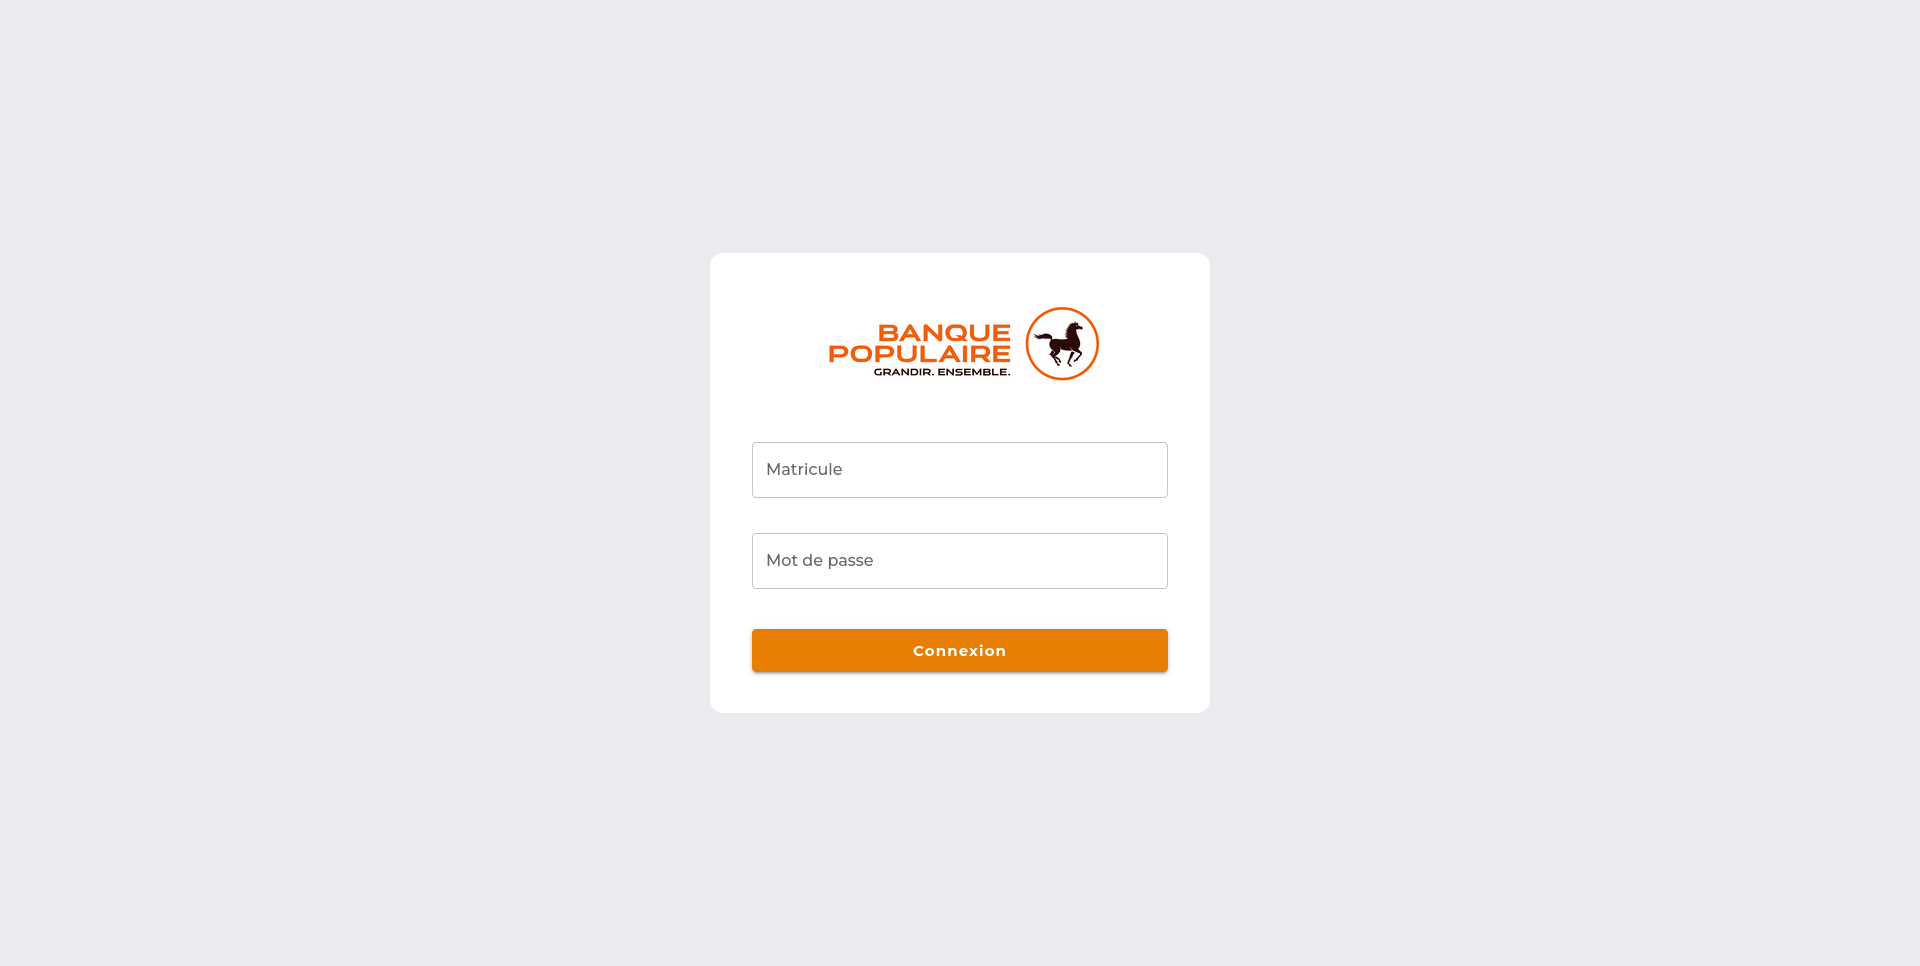
\includegraphics[height=.65\textwidth, angle=90]{images/guis/login.png}
    \caption{Page d'authentification}
\end{figure}


\clearpage



\subsection{Gestion des paramètrages}

\noindent Afin de permettre une certaine adaptabilité du registre de traitement aux besoins qui peuvent changer en matière des représentants du groupe, des directions de chaque représentant, de la nature des données traitées, et de la façon avec laquelle tous ces derniers seront exprimés, une page a été consacrée pour gérer l'ensemble des valeurs pouvant être pris par tous les attributs de la fiche du traitement. \\


\begin{figure}[H]
    \centering
    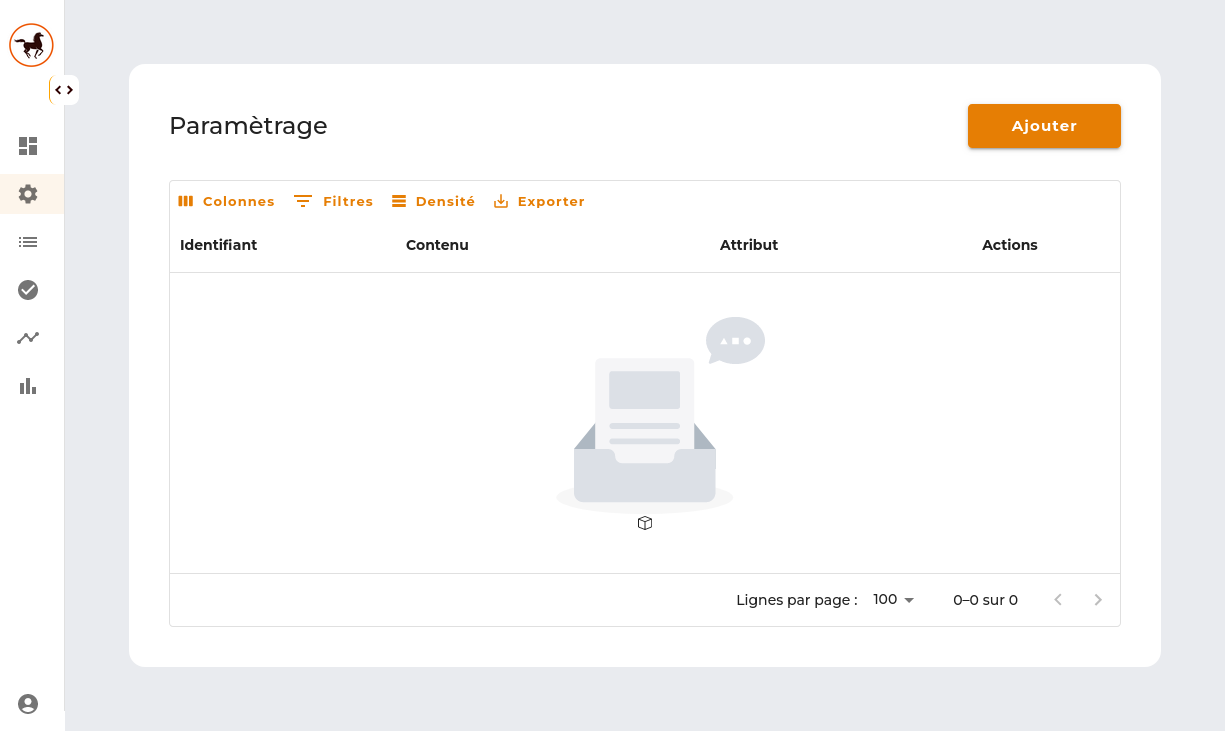
\includegraphics[width=\textwidth]{images/guis/parametrage/initial.png}
    \caption{Page de paramétrage}
\end{figure}

\vspace{.2cm}

\noindent La page est composée d'un tableau affichant l'ensemble de ces valeurs, ainsi qu'un bouton qui en permet l'extension en exposant un formulaire dont les champs décrivent les caractéristiques de la valeur à ajouter. \\

\noindent Initialement, et avant tout ajout d'une nouvelle valeur, le tableau est naturellement vide et un "placeholder" démontrant l'absence de valeurs est affiché.

\noindent Les colonnes du tableau décrivent des caractéristiques des valeurs tels que l'identifiant, le contenu, ainsi que le nom d'attribut auquel la valeur appartient. Pour chaque valeur, le tableau expose une dernière colonne qui permet d'effectuer certains actions sur la valeur en question. Notamment, la modification et la désactivation. \\

\noindent Le tableau comporte également une barre d'outil qui permet de limiter le nombre des colonnes affichées, de filtrer les valeurs du tableau, de modifier la taille des lignes, ainsi que d'exporter l'ensemble des valeurs derrière le tableau en un fichier csv.
\clearpage

\noindent Lors du clique sur le bouton libellé "Ajouter", un formulaire en "Modal" est affiché. Initialement, le formulaire impose une sélection de l'attribut à paramétrer. Suite à cette sélection, un nombre additionnel de champs est affiché qui dépend de la nature de l'attribut choisi. Pour la fiche du traitement on distingue trois types d'attributs: \\

\begin{itemize}
    \item  \textbf{Indépendants}: Ils constituent une majorité des attributs de la fiche, et ils présentent aucune association avec le reste des attributs. Le paramétrage de ces attributs, donc, naturellement, nécessite uniquement la valeur à ajouter. De ce fait, lors de la sélection d'un de ces attributs, un seul champ est ajouté, celui destiné à la nouvelle valeur de l'attribut;
    \item \textbf{Associés}: Ces derniers présentent des associations avec d'autres attributs, et donc, par exemple, le paramétrage d'un attribut ayant un association ManyToOne avec un autre attribut, nécessite non-uniquement la nouvelle valeur de l'attribut à paramétrer, mais également la valeur de l'attribut de l'autre coté de l'association;
    \item \textbf{Composés}: Sont composés de plusieurs attributs, qui pevent eux memes etre composés, associés, ou/et indépendants. La paramétrage de ces attributs nécessite tout ce qui est nécessaire pour le paramètrage des attributs composants.
\end{itemize}




\begin{figure}[H]
    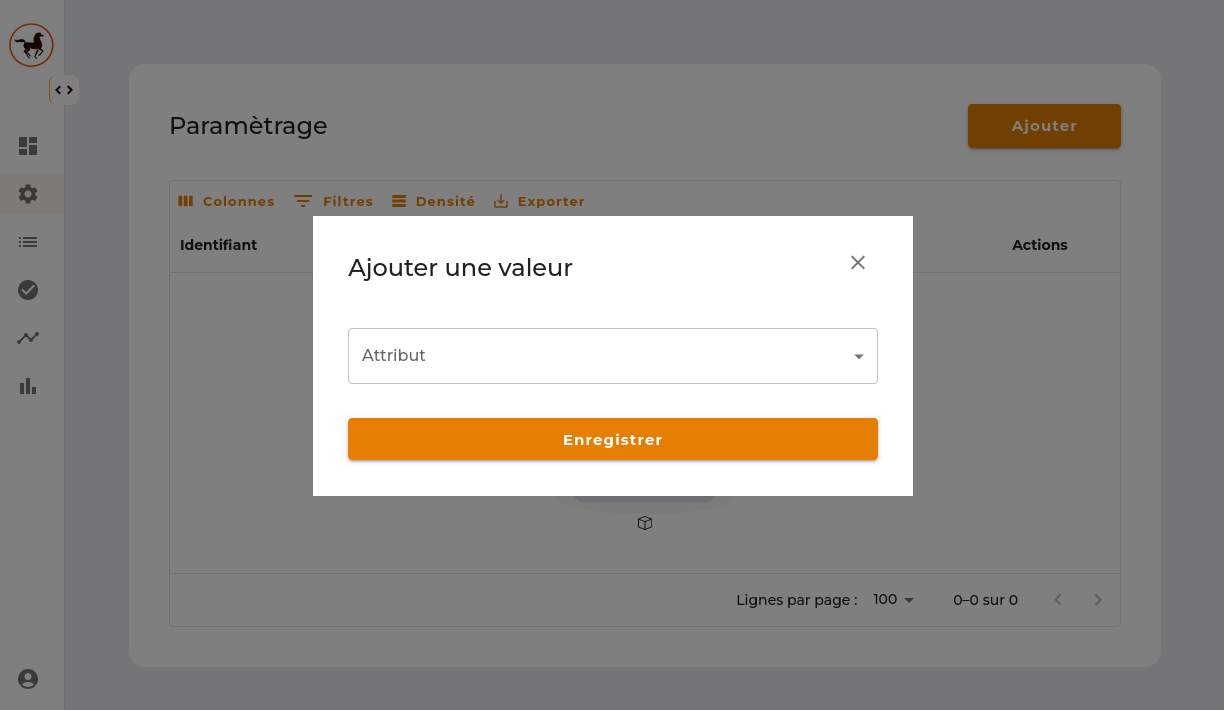
\includegraphics[width=.7\textwidth]{images/guis/parametrage/form-initial.png}
    \caption{Page de paramétrage}
\end{figure}

\begin{figure}[H]
    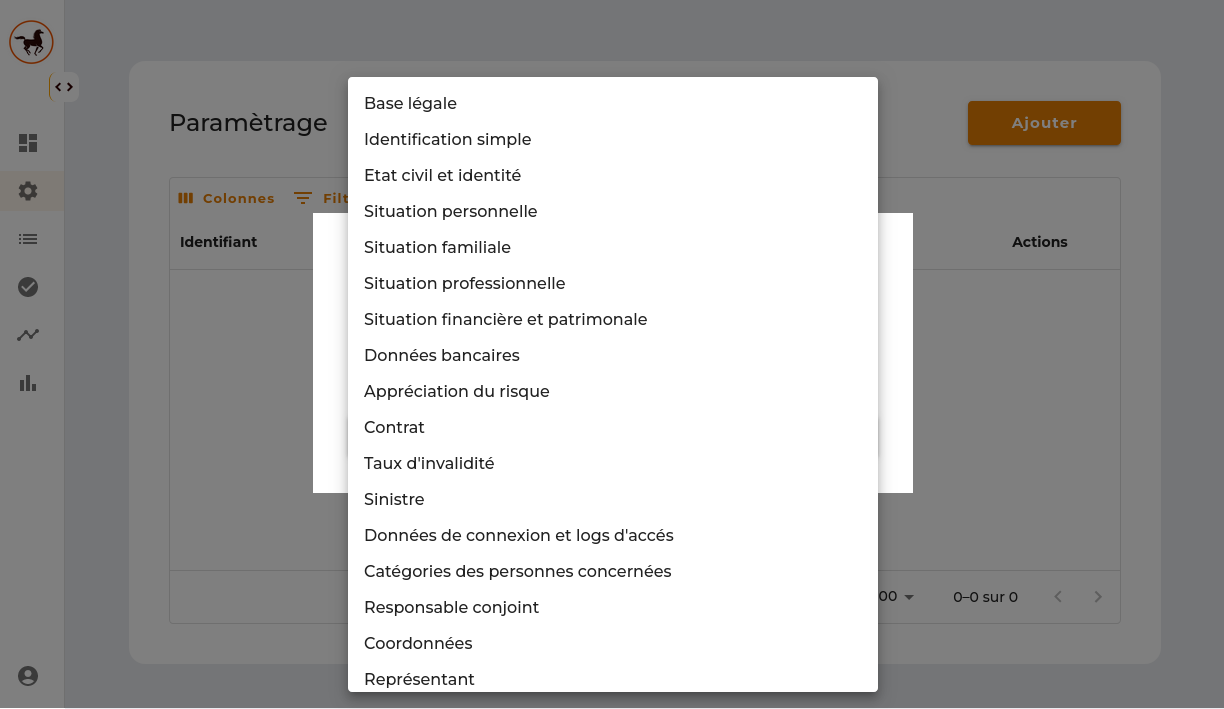
\includegraphics[width=.7\textwidth, right]{images/guis/parametrage/form-attribute-selection.png}
    \caption{Page de paramétrage}
\end{figure}

\clearpage

\noindent La figure ci-dessous illustre un exemple de paramétrage des attributs qualifiés "associés". L'attribut est nommé "Base légale" et ne dispose d'aucune association avec les autres attributs de la fiche. Dans cette figure, le formulaire est composé uniquement de deux champs, celui dédié à l'attribut à paramètrer, et celui dédié à sa nouvelle valeur, égale à "base1" dans le présent cas. \\

\begin{figure}[H]
    \centering
    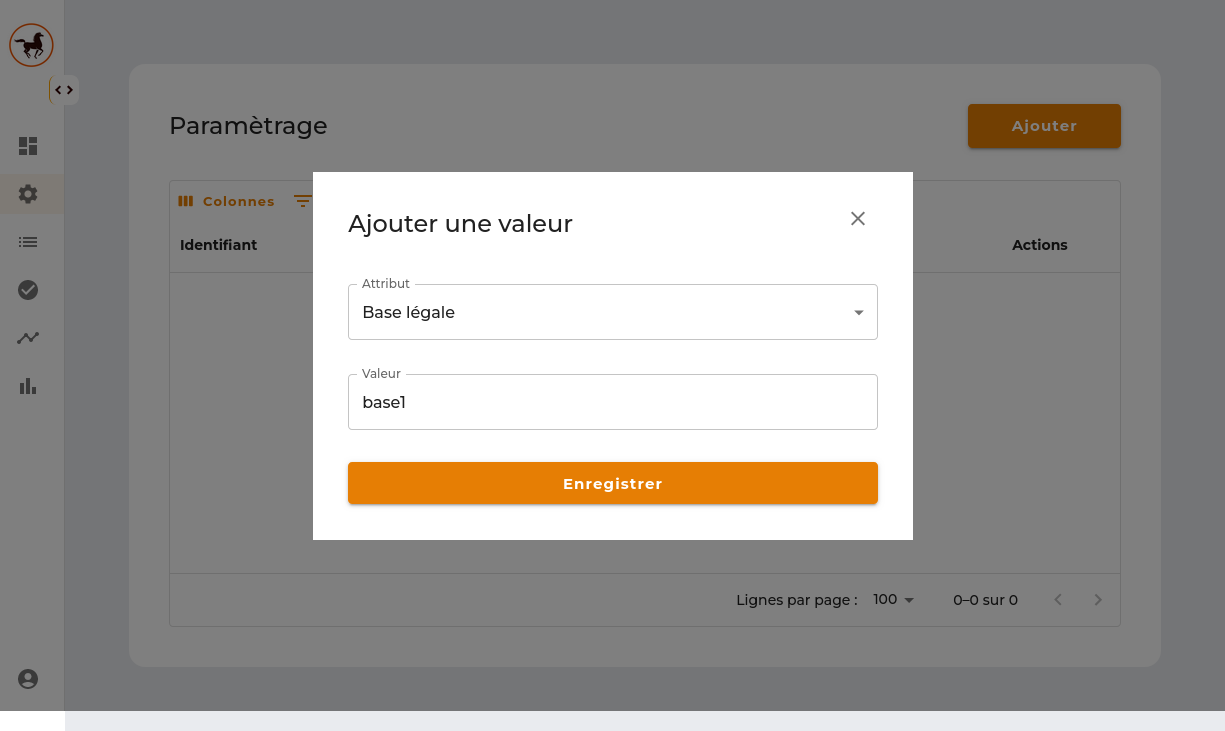
\includegraphics[width=\textwidth]{images/guis/parametrage/form-independent-attribute.png}
    \caption{Page de paramétrage}
\end{figure}

\clearpage

\noindent Pour les attributs qualifiés "associés", le formulaire s'adapte lors de la sélection de l'attribut en exposant des champs destinées aux valeurs des attributs avec lesquels il présente une association. \\

\noindent Par exemple, l'attribut nommé "Representant" dispose de deux associations "OneToMany" avec les attributs "Direction" et "Logiciel". De ce fait, la sélection de "Representant" dans le champs libellé "Attribut" résulte en l'ajout de deux champs supplémentaire, un libellé "Direction" et l'autre "Logiciel". \\


\begin{figure}[H]
    \centering
    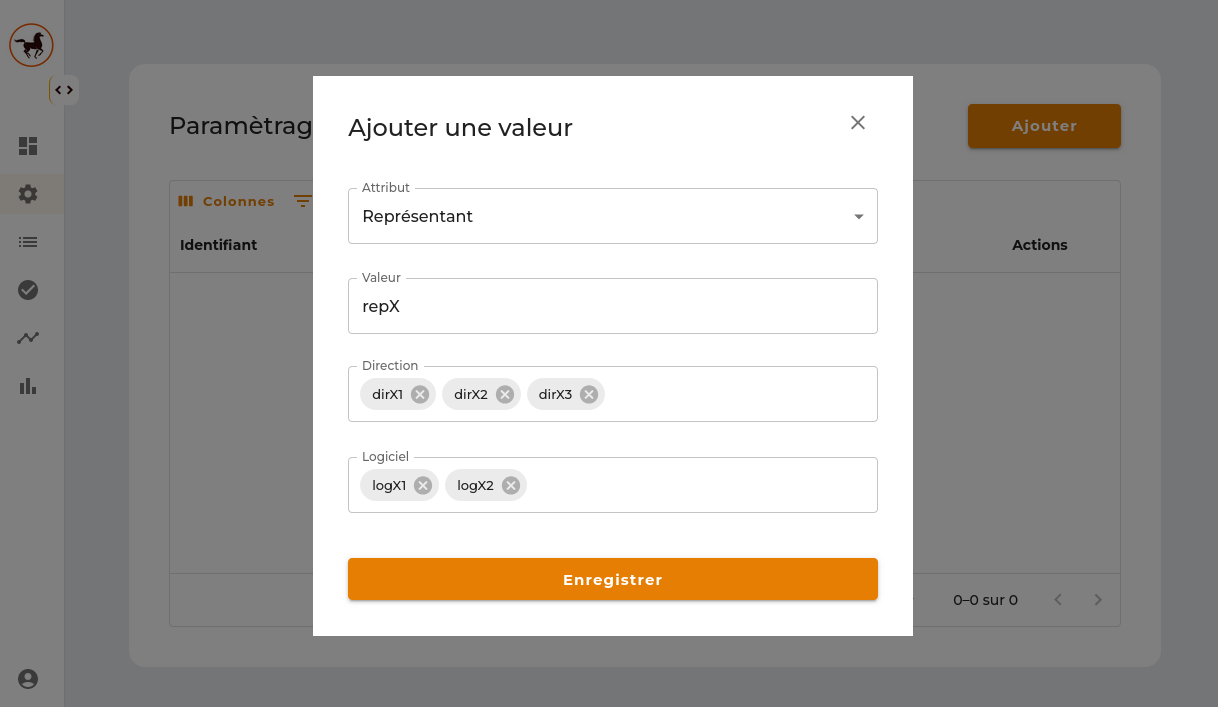
\includegraphics[width=\textwidth]{images/guis/parametrage/form-parent-attribute.png}
    \caption{Page de paramétrage}
\end{figure}

\noindent Du fait de la nature "OneToMany" de l'association dont dispose l'attribut "Représentant" avec les autres attributs, les valeurs de ces derniers ne sont pas obligatoires dans le formulaire. \\

\noindent La figure ci-dessus présente un cas d'utilisation dont l'utilisateur souhaite ajouter un représentantr dont la valeur est "repX", dont les directions sont "dirX1", "dirX2", et "dirX3", et dont les logiciels sont "logX1" et "logX2". Suite à cet ajout, le tableau des valeurs est populé par la valeur du nouveau représentant, ainsi que les valeurs des attributs avec lequel il dispose d'une association "OneToMany".




\clearpage

\begin{figure}[H]
    \centering
    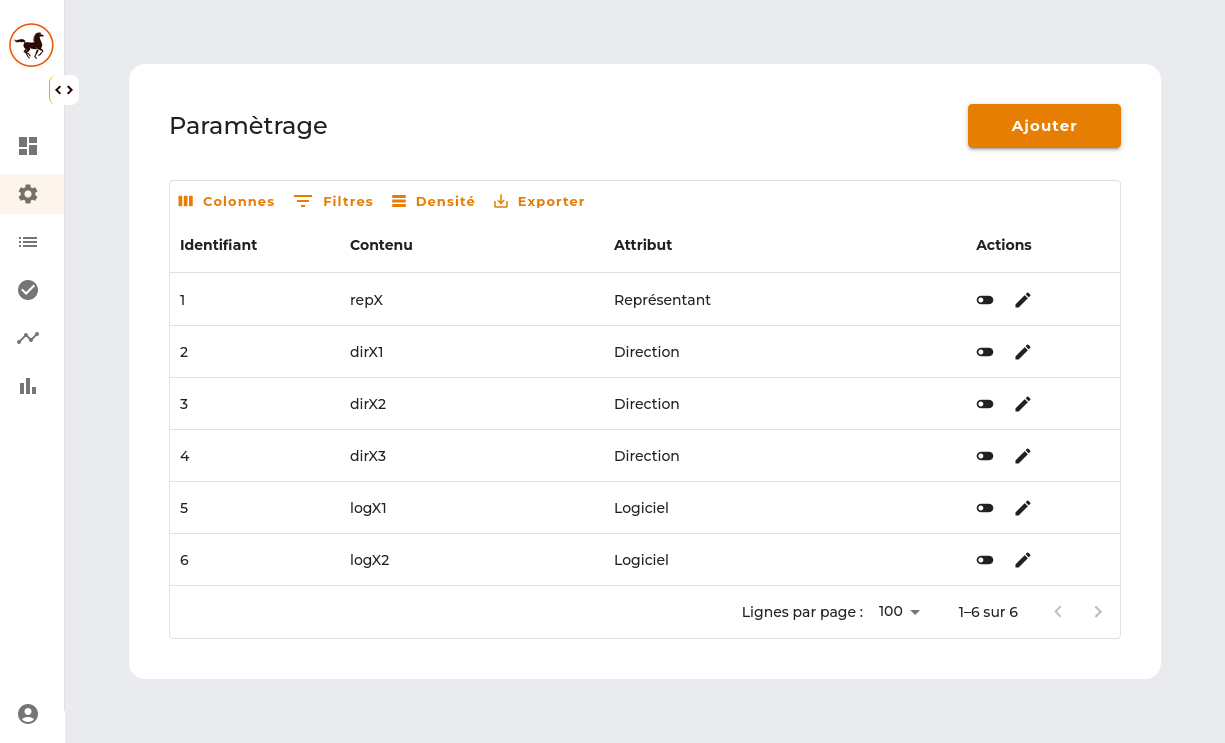
\includegraphics[width=\textwidth]{images/guis/parametrage/table-post-parent-saved.png}
    \caption{Page de paramétrage}
\end{figure}


\noindent Si un besoin se présente d'ajouter une nouvelle direction au représentant "repX", l'utilisateur peut faire usage du même formulaire en sélectionnant "Direction" comme attribut. Cette fois-ci, le formulaire s'adapte en exposant un champ dédié à la valeur du répresentant avec lequel la nouvelle direction sera associée. Vu que l'association Direction -\> Représentant est "ManyToOne", la saisie de la valeur du représentant est obligatoire pour l'enregistrement de la nouvelle direction. 

\begin{figure}[H]
    \centering
    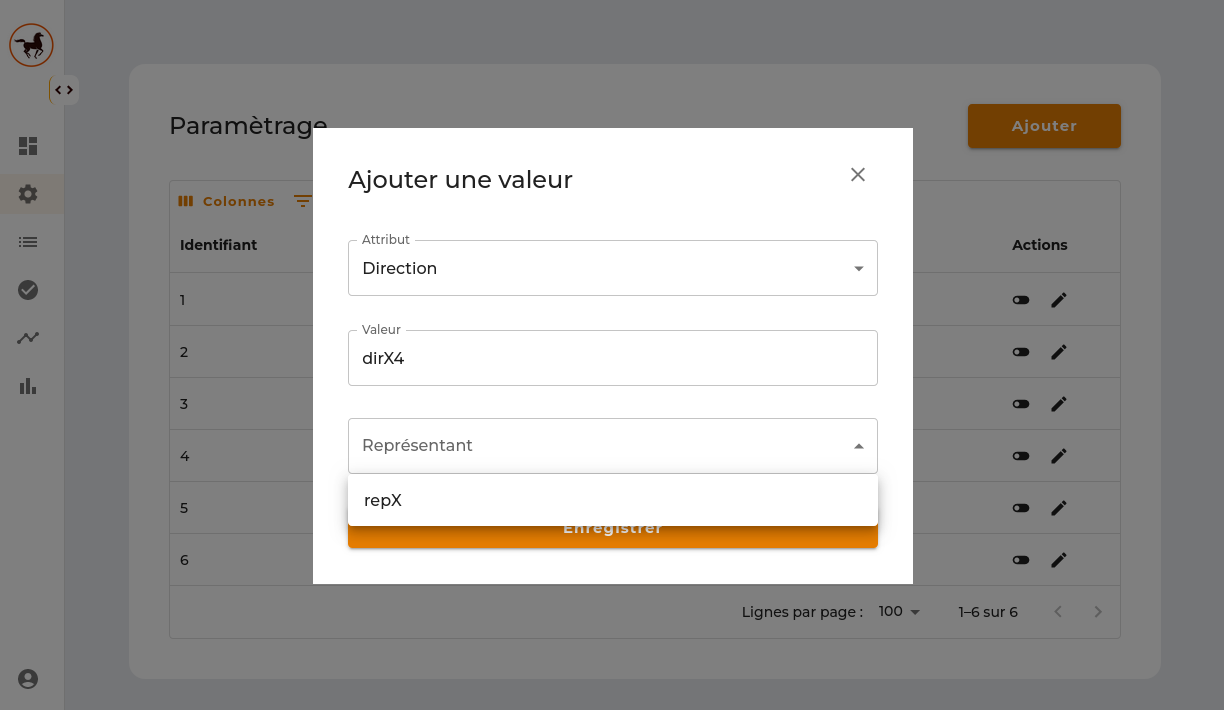
\includegraphics[width=\textwidth]{images/guis/parametrage/form-child1.png}
    \caption{Page de paramétrage}
\end{figure}

\clearpage

\noindent La figure 4.19 illustre le comportement du formulaire lors de la sélection de l'attribut "Direction". On remarque que le représentant "repX" précédemment enregistré figure dans l'ensemble des choix du champ libellé "Représentant". 

\noindent Le même s'applique lors du paramétrage de l'attribut "Logiciel":

\begin{figure}[H]
    \centering
    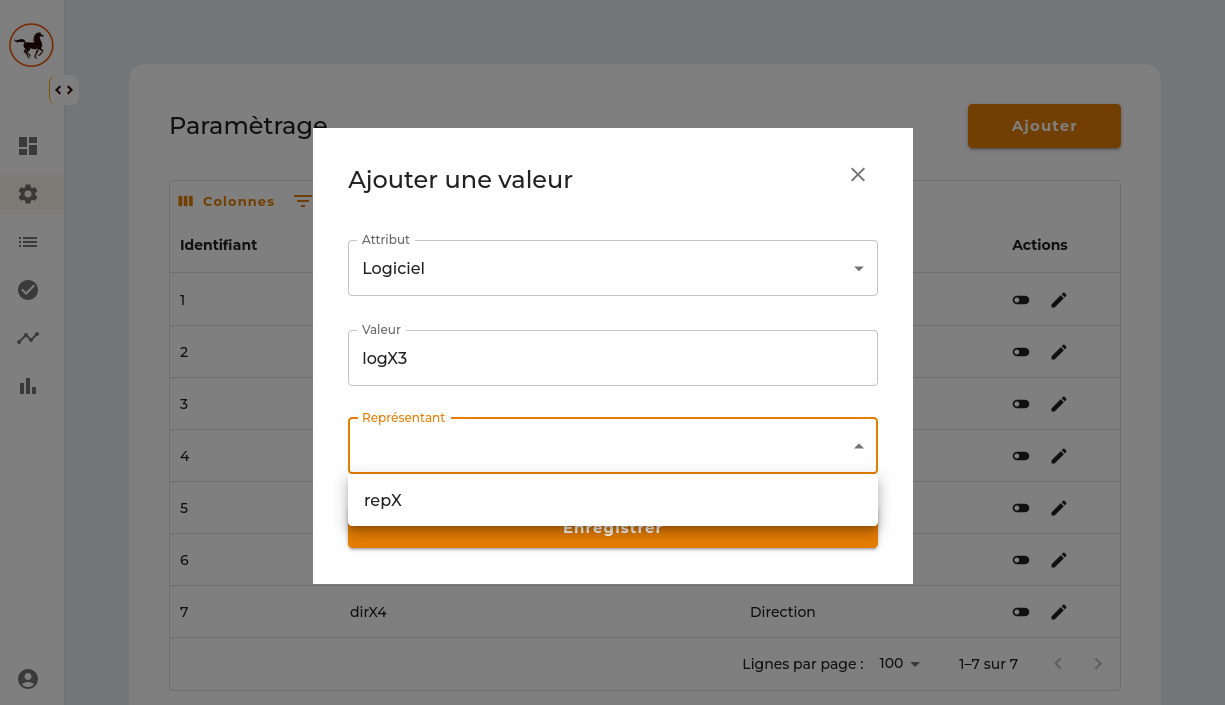
\includegraphics[width=.8\textwidth]{images/guis/parametrage/form-child2.png}
    \caption{Page de paramétrage}
\end{figure}


\noindent Suite à l'enregistrement de ces valeurs, le tableau s'adapte dynamiquement pour refleter les changements: \\

\begin{figure}[H]
    \centering
    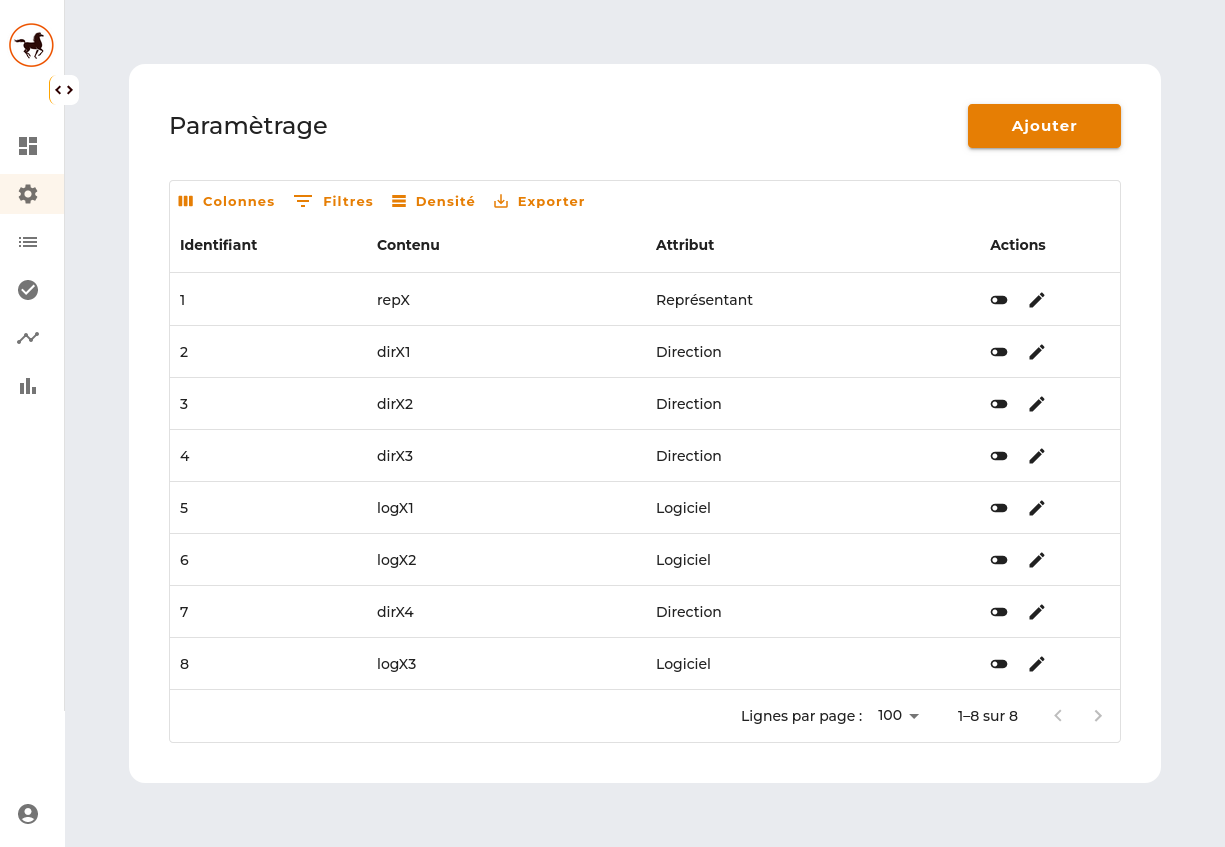
\includegraphics[width=\textwidth]{images/guis/parametrage/post-children-save-table.png}
    \caption{Page de paramétrage}
\end{figure}


\clearpage
\subsection{Ajout d'une fiche de traitement}

L'ajout d'une fiche de traitement se fait à travers un formulaire à plusieurs étapes dont chacune décrit un sous-ensemble des caractéristiques du traitement en question. Le choix d'utiliser un formulaire à plusieurs étapes originait de la nécessité d'avoir une vue détaillée du traitement des données, et ce afin d'exposer toutes les informations qui peuvent jouer un rôle dans l'évaluation de la conformité du traitement aux réglementations en matière de la protection des données à caractère personnel. \\

\noindent La première étape, libellée "Identification de la fiche", expose des champs qui permettent d'identifier le traitement en question, ses finalités, les différentes parties qui en portent la responsabilité, ainsi que des informations originaires de la CNDP. Dans cette partie, le remplissage des champs relatifs au représentant du responsable du traitement, de ses directions, ainsi que les logiciels à l'aide desquels le traitement va être effectué est obligatoire. Suite au remplissage de ces champs, le bouton "Suivant" devient actif et l'utilisateur peut naviguer à l'étape suivante. \\

\begin{figure}[H]
    \centering
    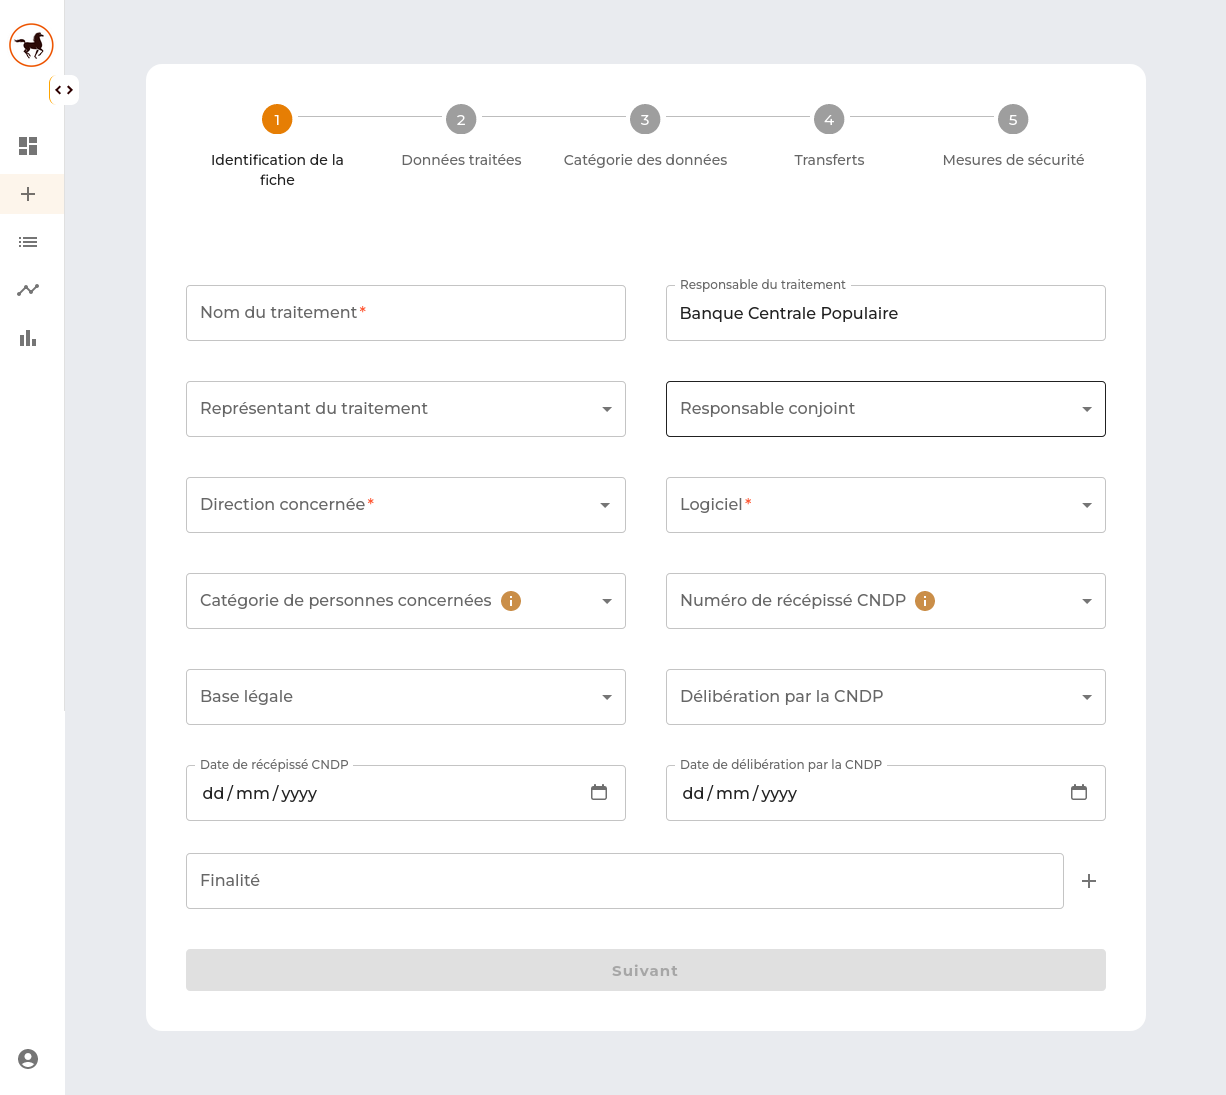
\includegraphics[width=\textwidth]{images/guis/nouvelle-fiche/nouvelle-fiche-1.png}
    \caption{Page d'ajout d'une fiche de traitement}
\end{figure}

\clearpage

\noindent La deuxième étape, libellée \textit{"Données traitées"}, concerne, comme le nom l'indique, la nature des données sur lesquels va opérer le traitement. Dans le but d'offrir une meuilleure repérabilité des données à traiter, une décomposition à 3 niveaux a été utilisée dont chaque type de données appartient à un super-type lui même ayant un super-type.

\begin{figure}[H]
    \centering
    \includegraphics[width=\textwidth]{images/guis/nouvelle-fiche/nouvelle-fiche-2-1.png} 
    \caption{Première section de la 2ème étape du formulaire de la fiche}
\end{figure}

\begin{figure}[H]
    \centering
    \includegraphics[width=\textwidth]{images/guis/nouvelle-fiche/nouvelle-fiche-2-2.png} 
    \caption{Deuxième section de la 2ème étape du formulaire de la fiche}
\end{figure}

\clearpage

\noindent La troisième étape, intitulée \textit{"Catégorie des données"}, regroupe des champs qui permettent de vérifier l'existence, et dans le cas positif de décrire, les catégories de données sensibles par nature (eg. opinions politiques, appartenance syndicale, conviction religieuse) ainsi que les données à caractère personnel constituant le sujet du traitement en question. Elle englobe également des champs destinés à la durée de conservation des données à traiter ainsi que les catégories des destinataires de ces données, s'il y en a. \\

\begin{figure}[H]
    \centering
    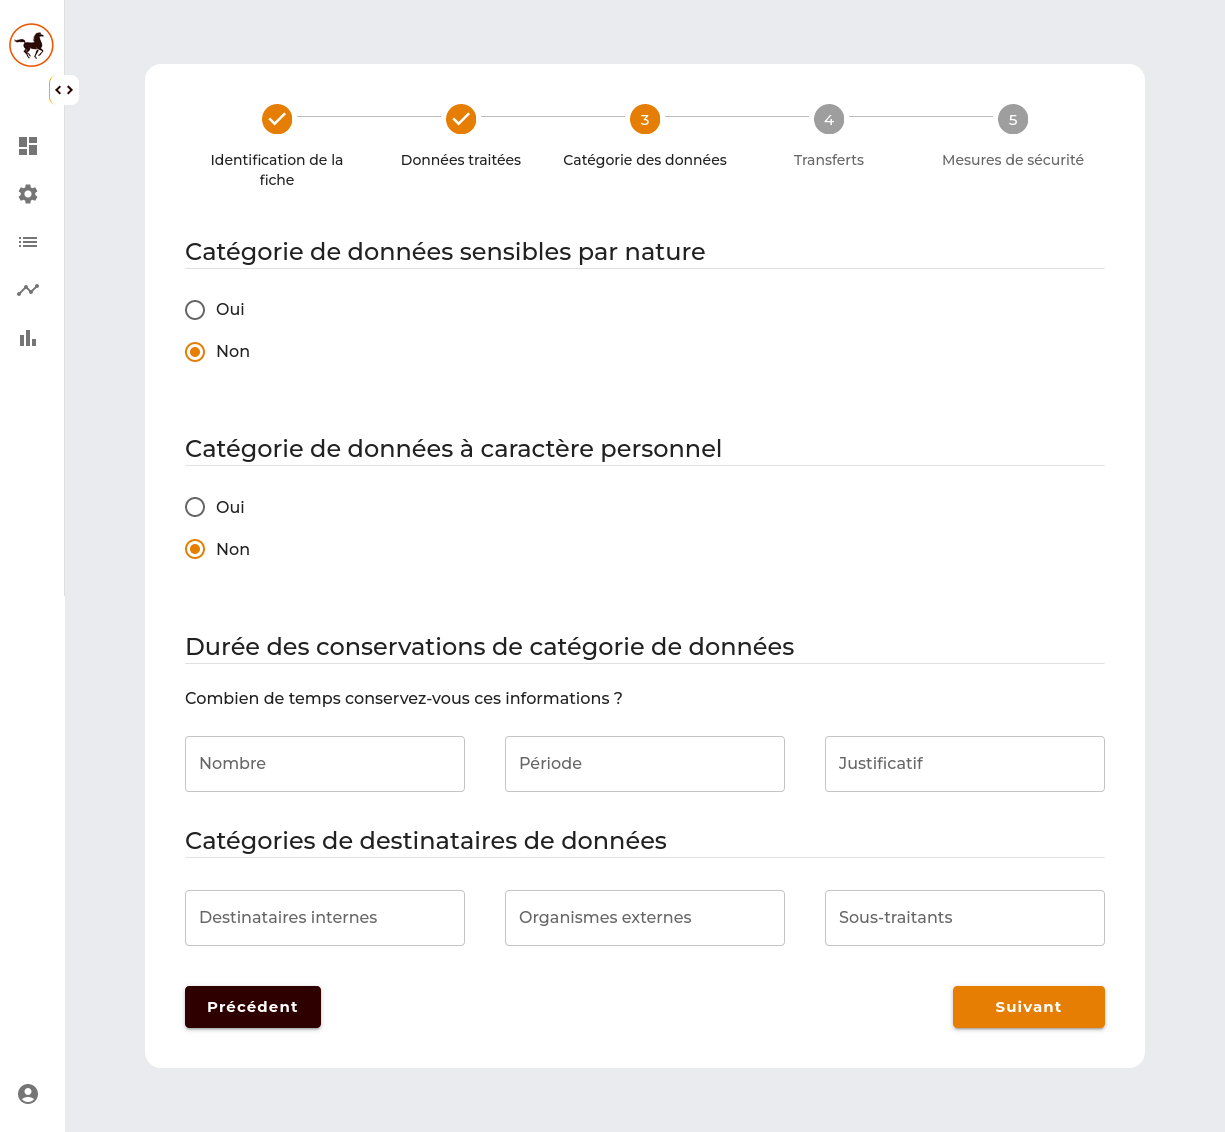
\includegraphics[width=\textwidth]{images/guis/nouvelle-fiche/nouvelle-fiche-3.png} 
    \caption{3ème étape du formulaire de la fiche}
\end{figure}
    
\clearpage

\noindent La quatrième étape, intitulée "Transferts," permet de spécifier si le traitement des données nécessite des transferts de celles-ci en dehors du Maroc ou de l'Union Européenne. Cette étape est cruciale pour assurer la conformité avec les réglementations locales et internationales sur la protection des données. Elle oblige les responsables du traitement à indiquer clairement les destinations des données et à vérifier que ces transferts respectent les normes de sécurité et de confidentialité en vigueur, garantissant ainsi la protection des droits des personnes concernées. \\

\begin{figure}[H]
    \centering
    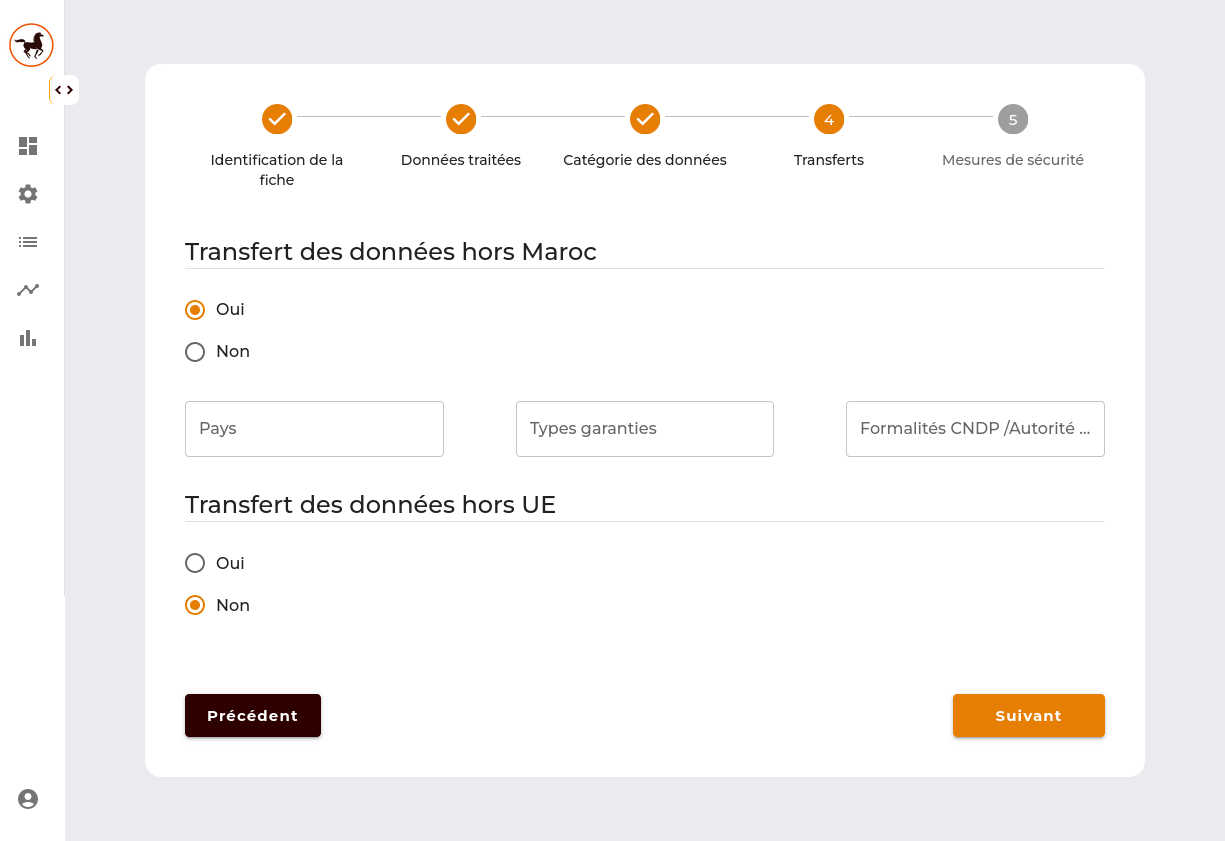
\includegraphics[width=\textwidth]{images/guis/nouvelle-fiche/nouvelle-fiche-4.png} 
    \caption{4ème étape du formulaire de la fiche}
\end{figure}

\clearpage

\noindent 
La dernière étape, \textit{"Mesures de sécurité"}, décrit l'ensemble des mesures à prendre afin d'assurer la confidentialité des données à traiter. Cette étape expose des champs dont chacun concerne une mesure spécifique de sécurité. L'utilisateur est censé ajouter, pour chaque mesure prise dans le contexte du traitement, des détails qui permettent de donner une vue plus compréhensive des efforts entrepris dans le contexte spécifique de la mesure en question. \\


\begin{figure}[H]
    \centering
    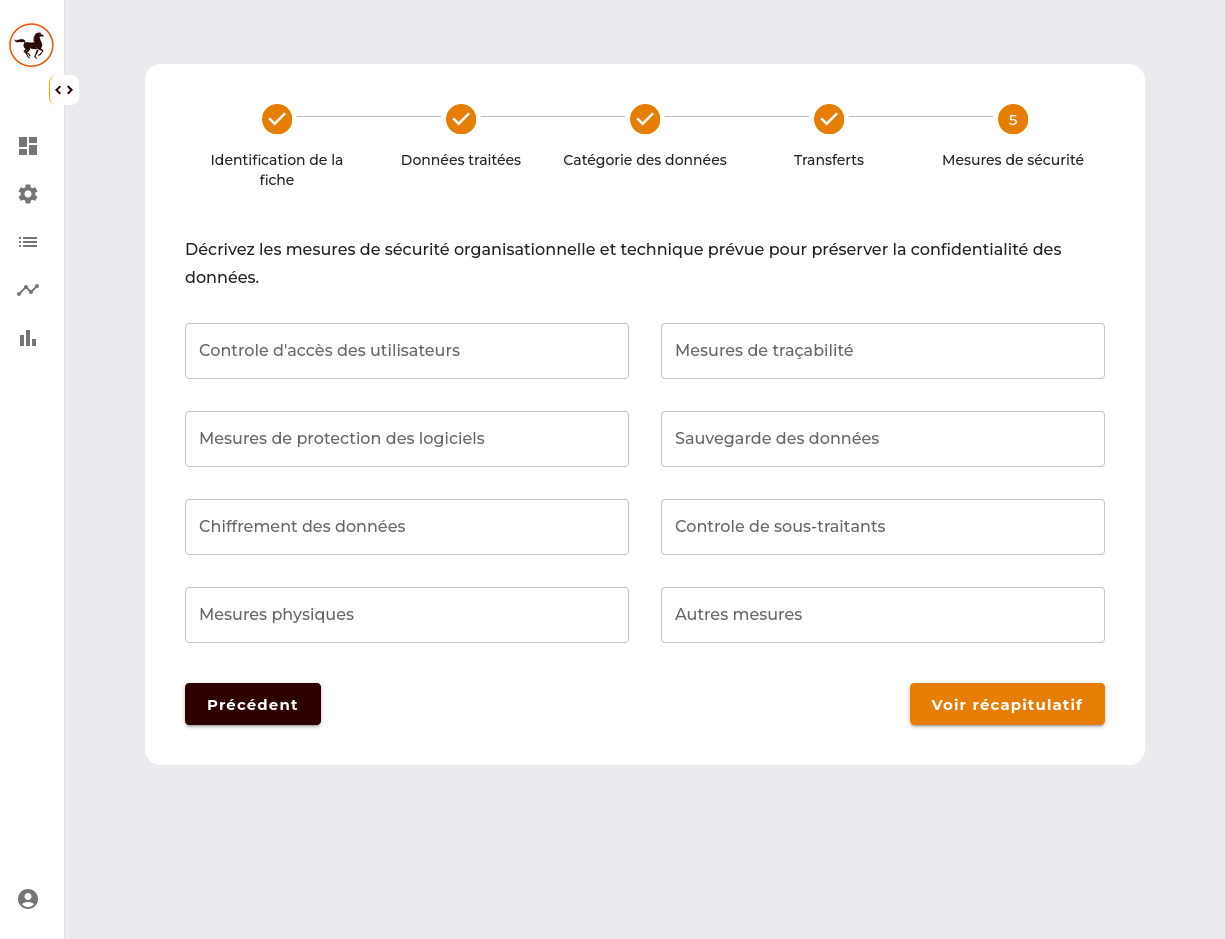
\includegraphics[width=\textwidth]{images/guis/nouvelle-fiche/nouvelle-fiche-5.png} 
    \caption{5ème étape du formulaire de la fiche}
\end{figure}

\noindent En vertu du coup élevé en cas de mal-saisie, le bouton "Suivant" est remplacé par un bouton qui permet à l'utilisateur de visualiser un récapitulatif des informations saisies à propos du traitement tout au long du formulaire, ce qui permet d'effectuer une dernière validation avant de confirmer l'enregistrement de la fiche de traitement. \\

\clearpage


\subsection{Gestion des fiches de traitement}

La gestion des fiches de traitement en matière de consultation, de modification, de suivie, et de suppression se fait à travers une page exposant l'ensemble des fiches du registre de traitement ainsi que les opérations pouvant être appliqués sur chaque fiche. \\

\noindent A l'exception de l'agent d'habilitation, tous les utilisateurs peuvent accéder à cette interface. Bien que l'accés à l'interface n'est pas totalement limité, le contenu de celle-ci s'adapte de manière à refleter les responsabilités et les autorisations de chaque acteur. \\

\noindent L'expert métier, étant rédacteur de la fiche du traitement, peut consulter cette interface pour suivre l'état d'avancement de ses propres fiches, d'y apporter des modifications, ou de supprimer une fiche du registre de traitement. Il est à noter que la suppression d'une fiche de traitement ne constitue pas une destruction totale de la fiche en question. La fiche continue à vivre dans la base de données pour des raisons de traçabilité mais elle cesse d'apparaître dans le tableau exposant l'ensemble des fiches du registre de traitement. Cette approche est nécessaire pour garantir un maximum de traçabilité et de transparence dans la gestion du registre de traitement. \\

\begin{figure}[H]
    \centering
    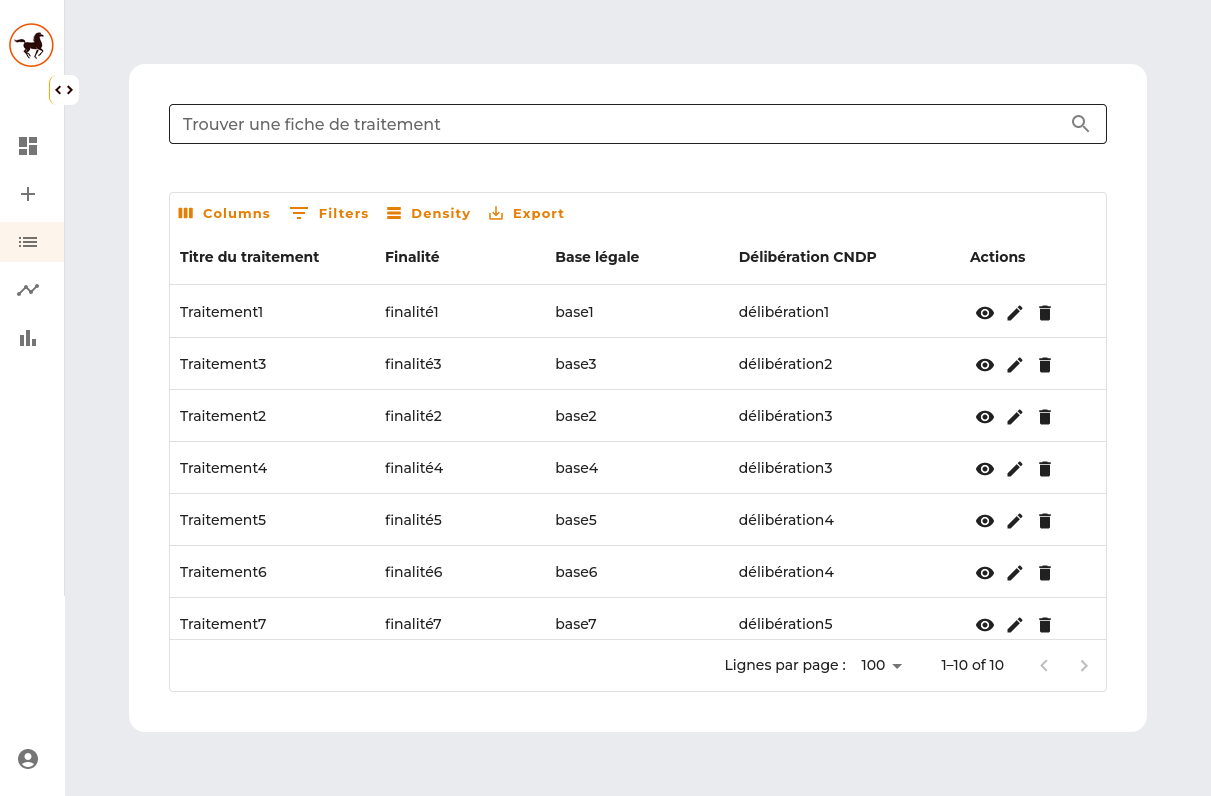
\includegraphics[width=\textwidth]{images/guis/fiches/fiches-em.png}
    \caption{Interface de gestion des fiche du point de vue de l'expert métier}
\end{figure}

\clearpage
 
\noindent 
Le RPO, chargé d'effectuer la première validation de la fiche de traitement, se sert de l'interface pour lister l'ensemble des fiches issues du représentant dont il fait partie. Pour chaque fiche du traitement, il peut y examiner le contenu et prendre une décision de valider, de rejeter, ou de retourner la fiche du traitement à l'expert métier. Chaque décision est enrichie d'un commentaire qui en sert de justification. \\

\begin{figure}[H]
    \centering
    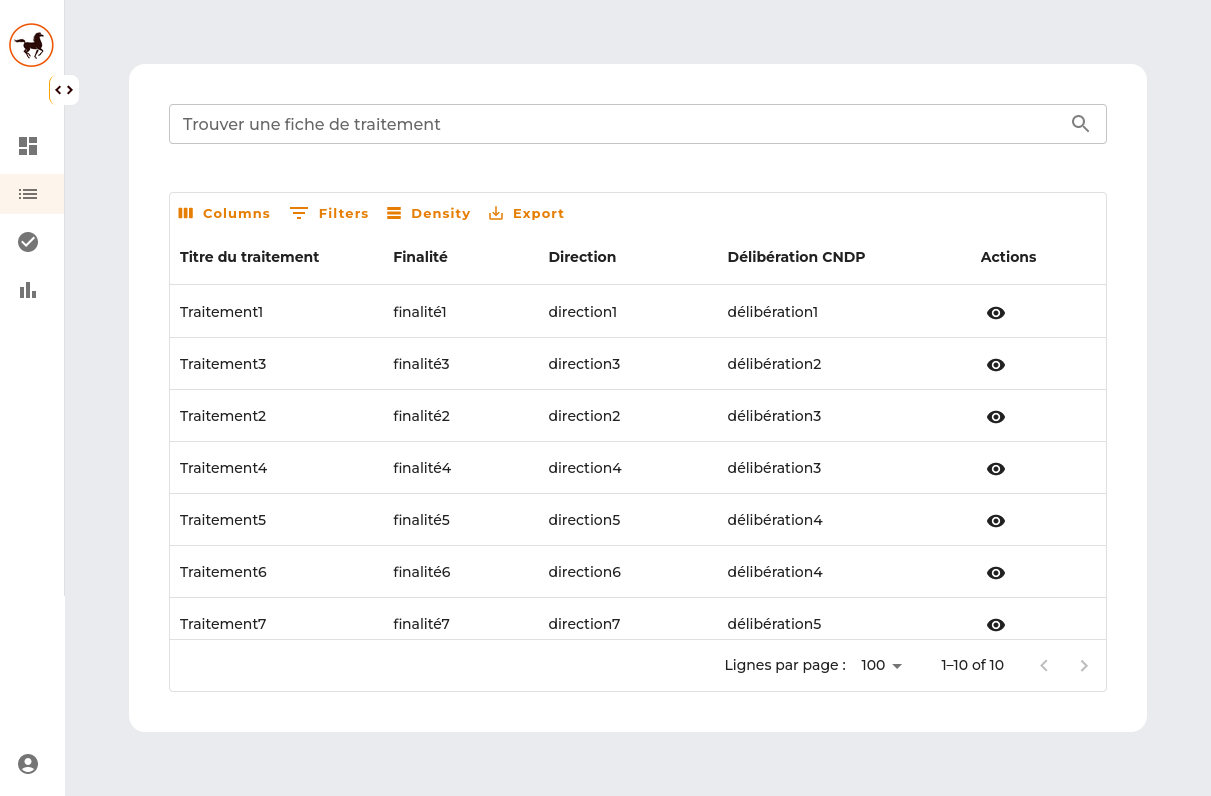
\includegraphics[width=\textwidth]{images/guis/fiches/fiches-rpo.png}
    \caption{Interface de gestion des fiche du point de vue du RPO}
\end{figure}

\vspace{.3cm}

\noindent Il est à noter que l'interface du point de vue du RPO, contrairement à celle destinée à l'expert métier, ne dispose pas de boutons pour la modification et la suppression des fiches de traitement. Conformément aux spécifications, ces opérations sont réservées uniquement à l'expert métier.  

\clearpage

\noindent L'interface s'adapte similairement aux responsabilités du DPO et du GDPO:

\begin{figure}[H]
    \centering
    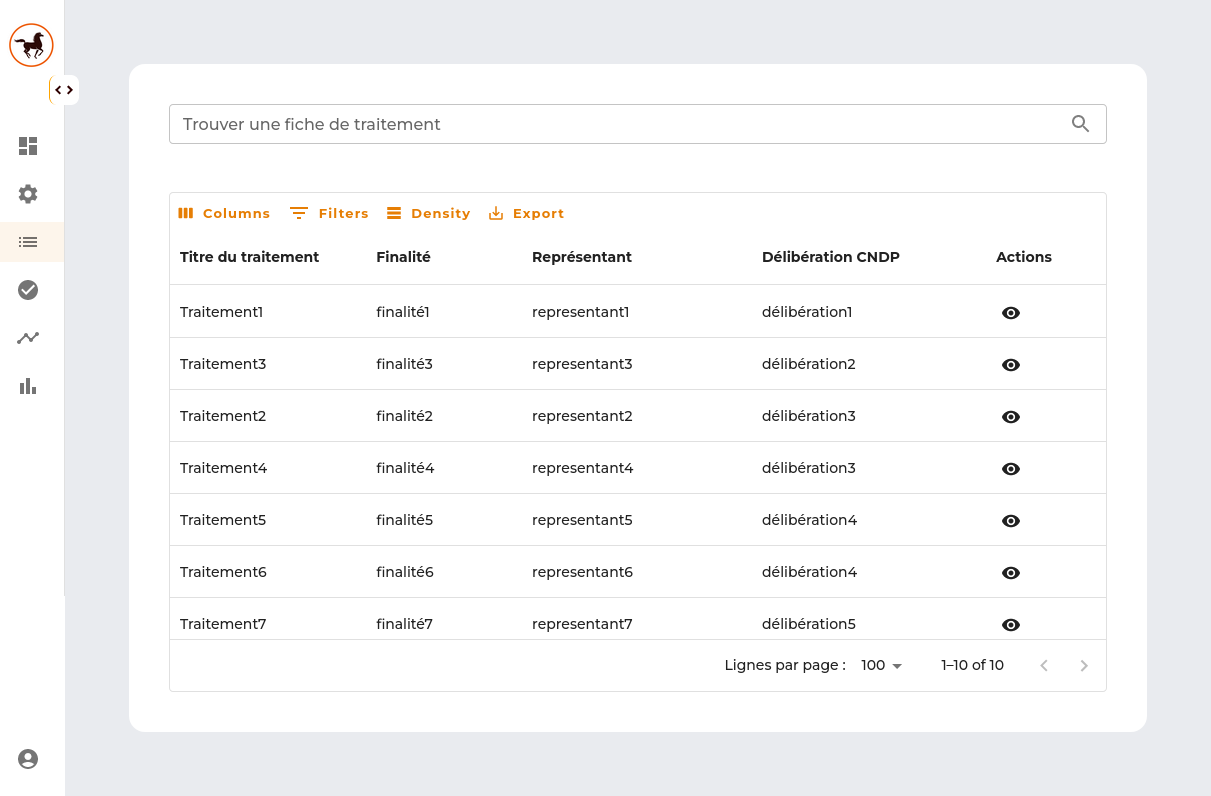
\includegraphics[width=\textwidth]{images/guis/fiches/fiches-dpo.png}
    \caption{Interface de gestion des fiche du point de vue du DPO}
\end{figure}

\begin{figure}[H]
    \centering
    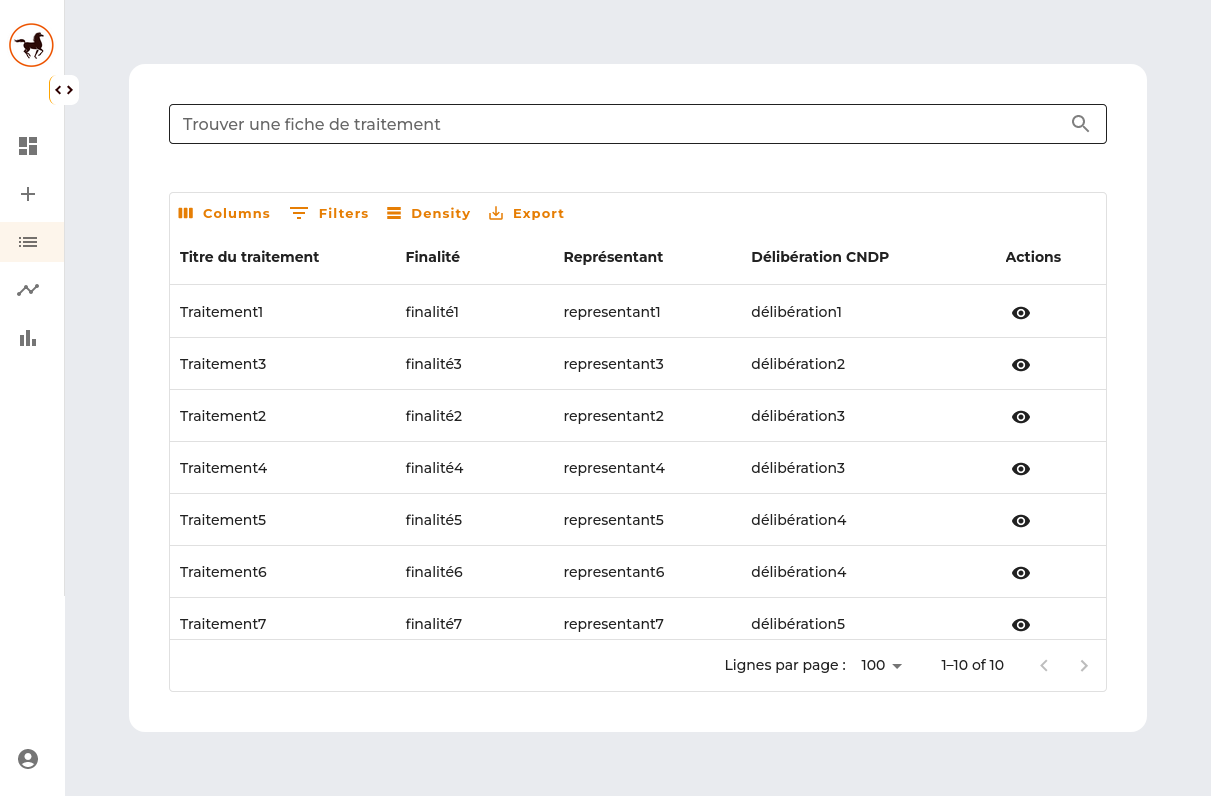
\includegraphics[width=\textwidth]{images/guis/fiches/fiches-gdpo.png}
    \caption{Interface de gestion des fiche du point de vue du GDPO}
\end{figure}

\clearpage

\subsection{Validation du traitement}

\begin{figure}[H]
    \centering
    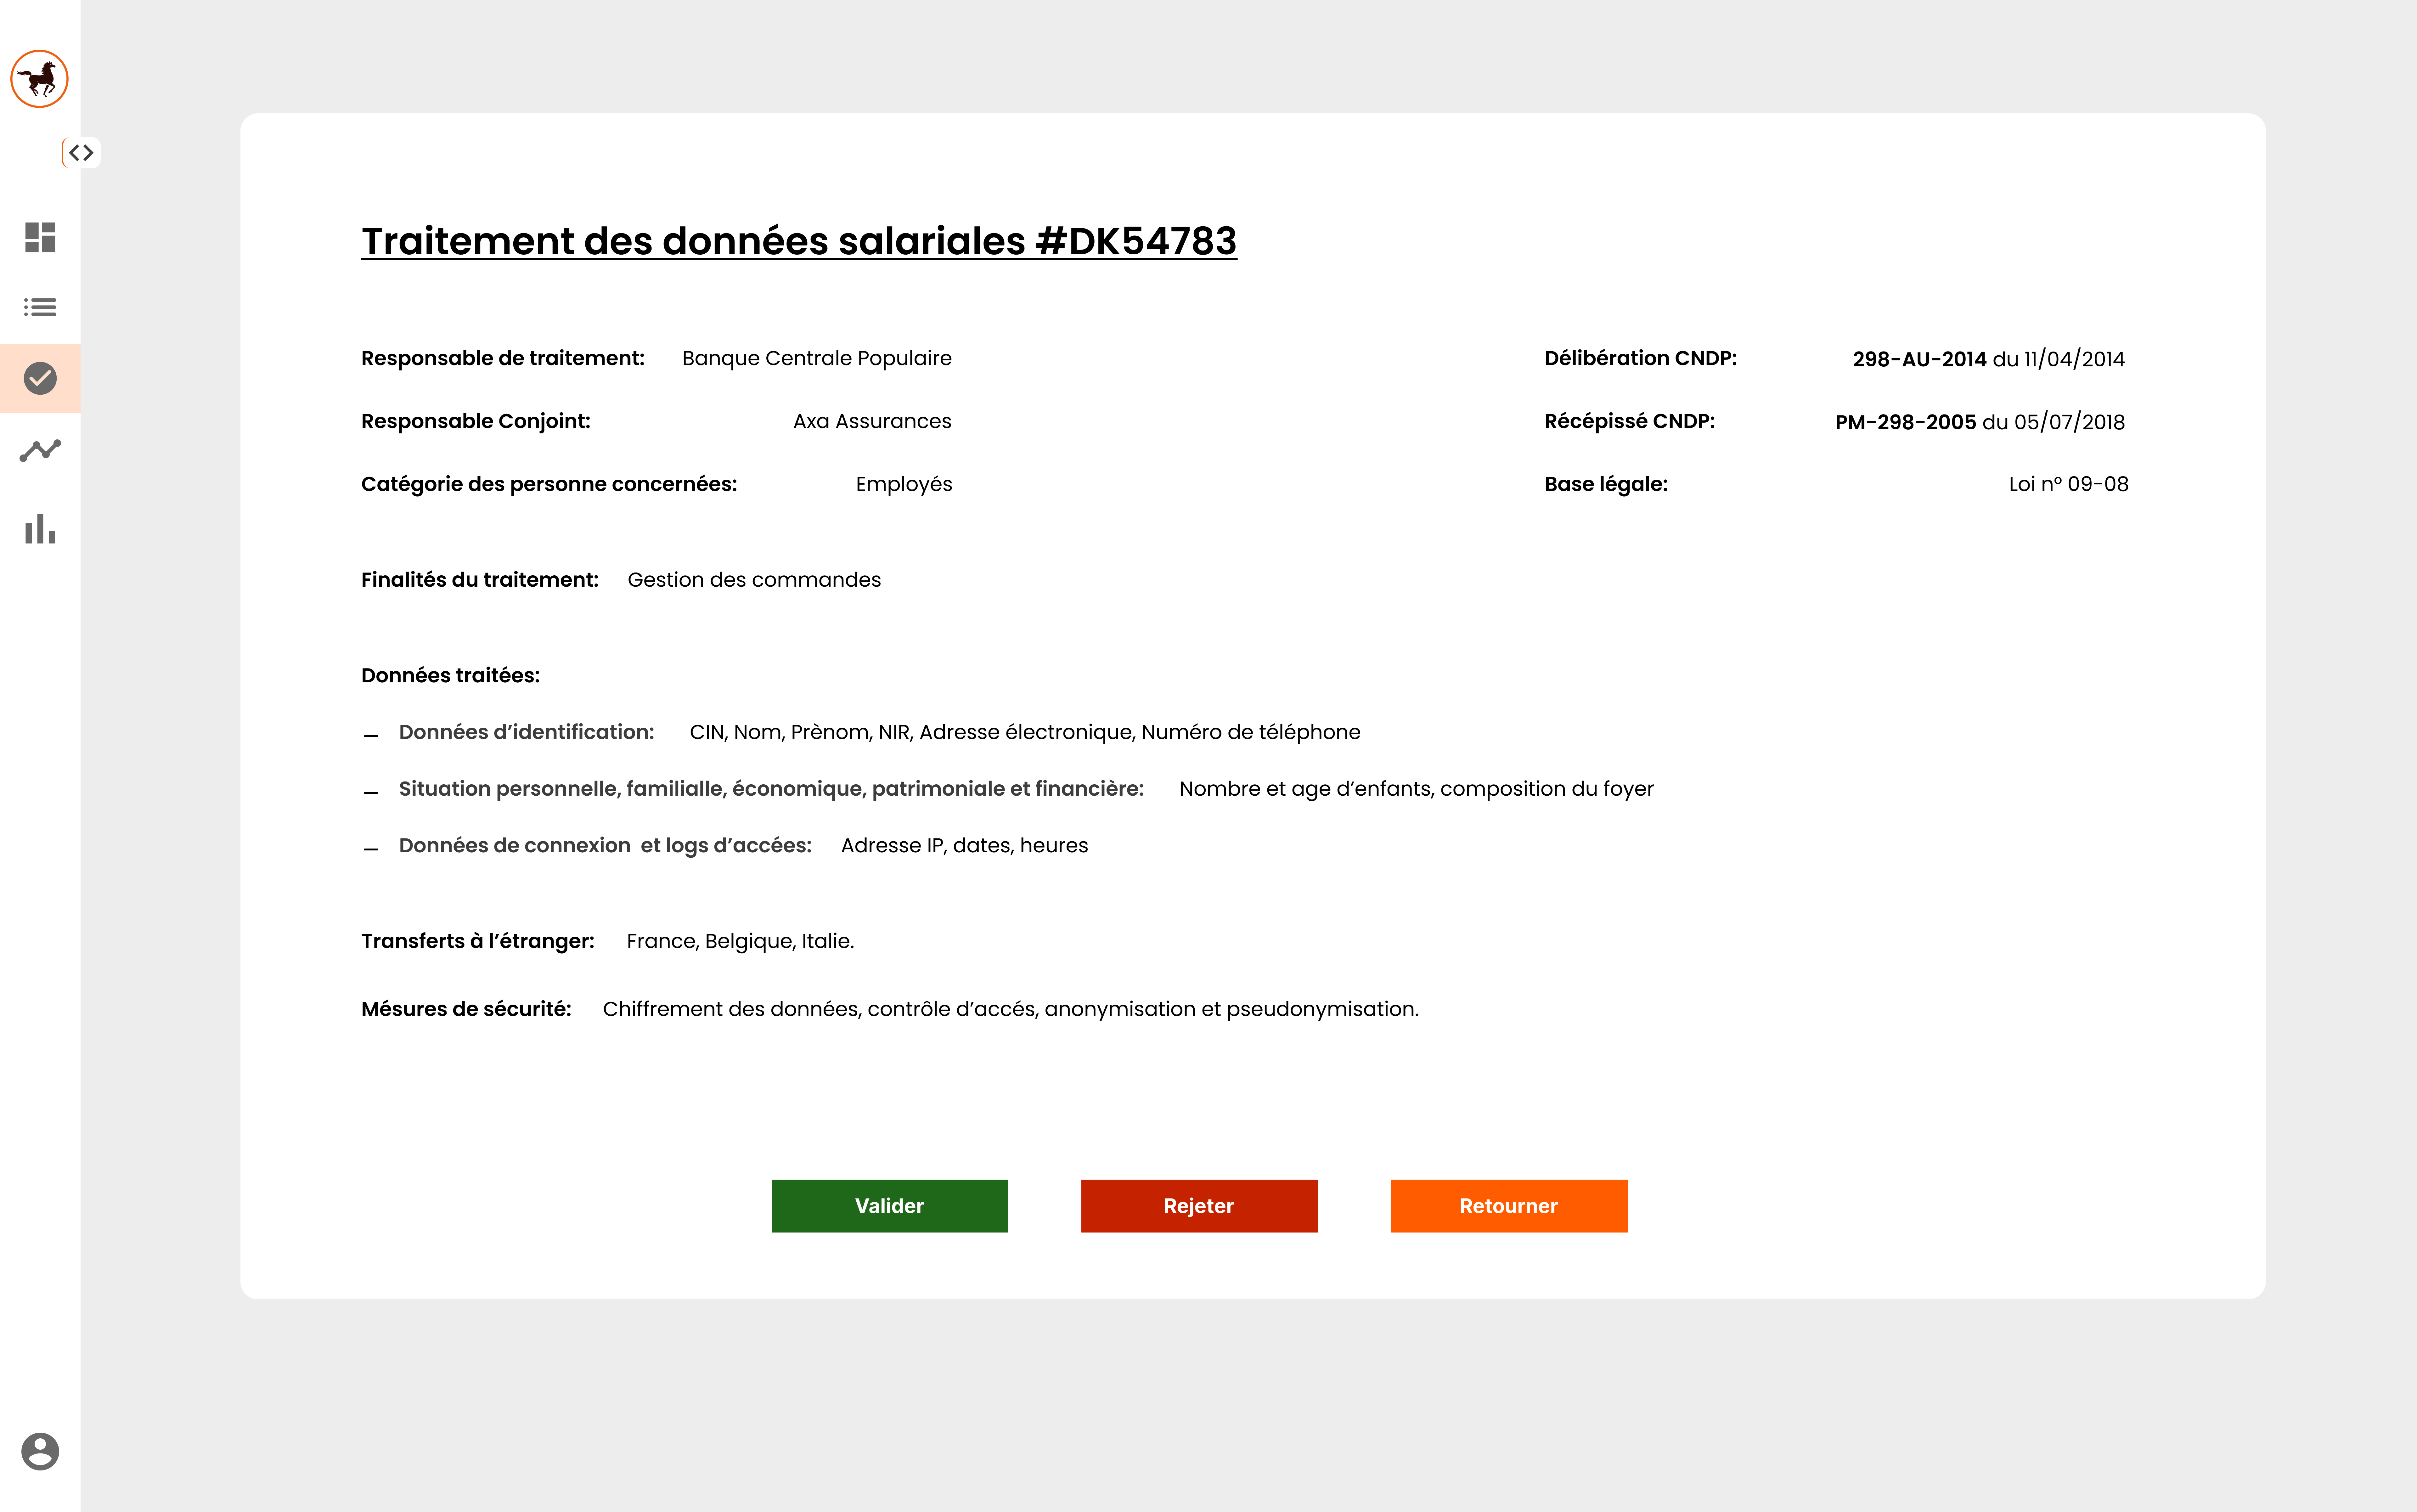
\includegraphics[height=.88\textwidth, angle=90]{images/guis/validation.png}
    \caption{Interface de gestion des utilisateurs}
\end{figure}

\clearpage

\subsection{Gestion des utilisateurs}

Similairement à la gestion des valeurs et des fiches de traitement, la gestion des utilisateurs se fait à travers une interface dédiée. L'interface comporte un tableau listant l'ensemble des utilisateurs et exposant des actions qui peuvent s'appliquer sur chaque utilisateur, ainsi q'un bouton qui permet d'ajouter de nouveaux utilisateurs au système d'automatisation du registre de traitement. \\

\noindent Conformément aux spécifications, uniquement l'agent d'habiliation possède le droit d'accéder et d'utiliser les fonctionnalités offertes par cette interfaces. \\

\begin{figure}[H]
    \centering
    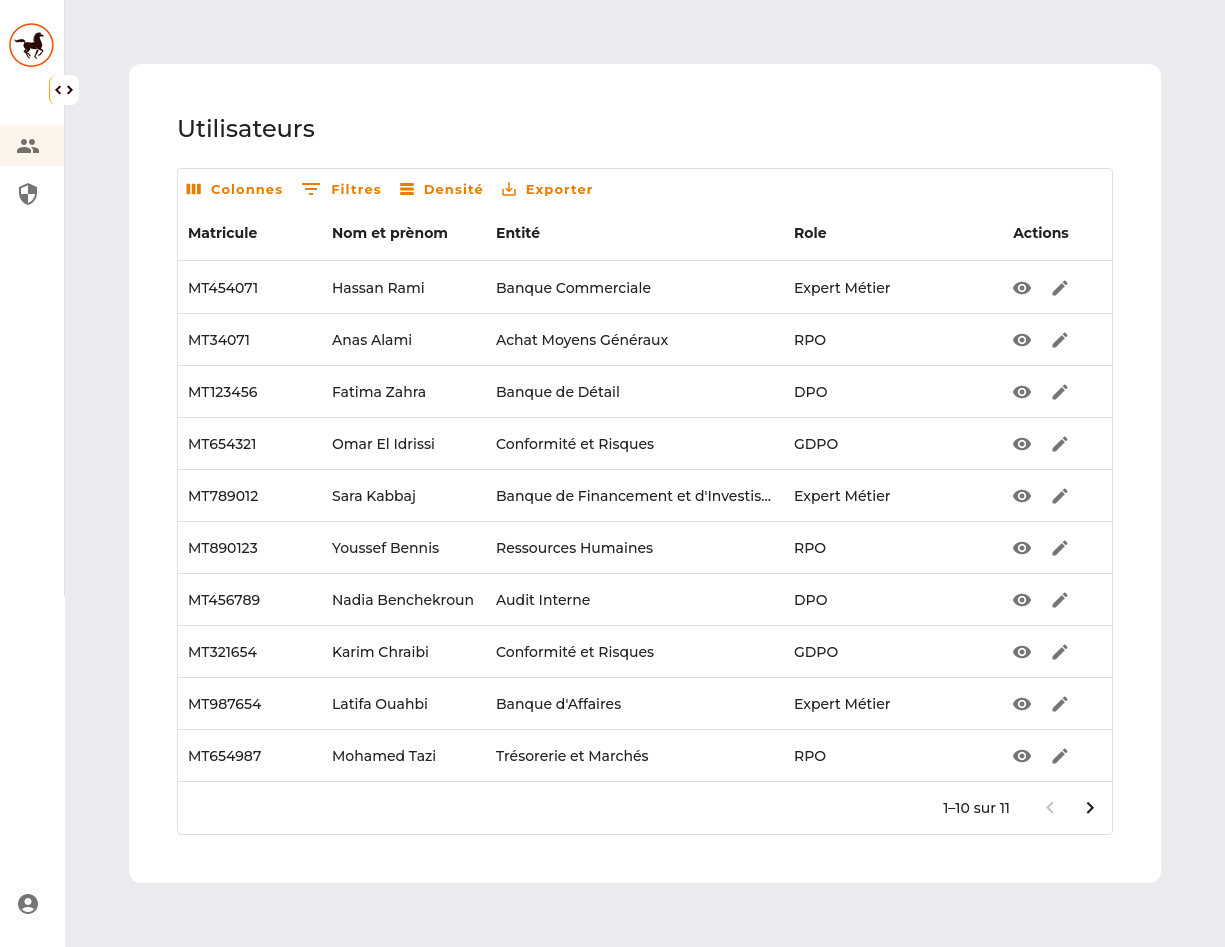
\includegraphics[width=\textwidth]{images/guis/utilisateurs.png}
    \caption{Interface de gestion des utilisateurs}
\end{figure}

\vspace{.3cm}

\noindent L'ajout de nouveaux utilisateurs se fait à traver un formulaire en "Modal" qui s'affiche une fois le bouton "Ajouter" est cliqué. Le formulaire permet d'insérer la matricule de l'utilisateur, son nom et prénom, ainsi que le rôle qu'il va jouer dans l'application.

\begin{figure}[H]
    \centering
    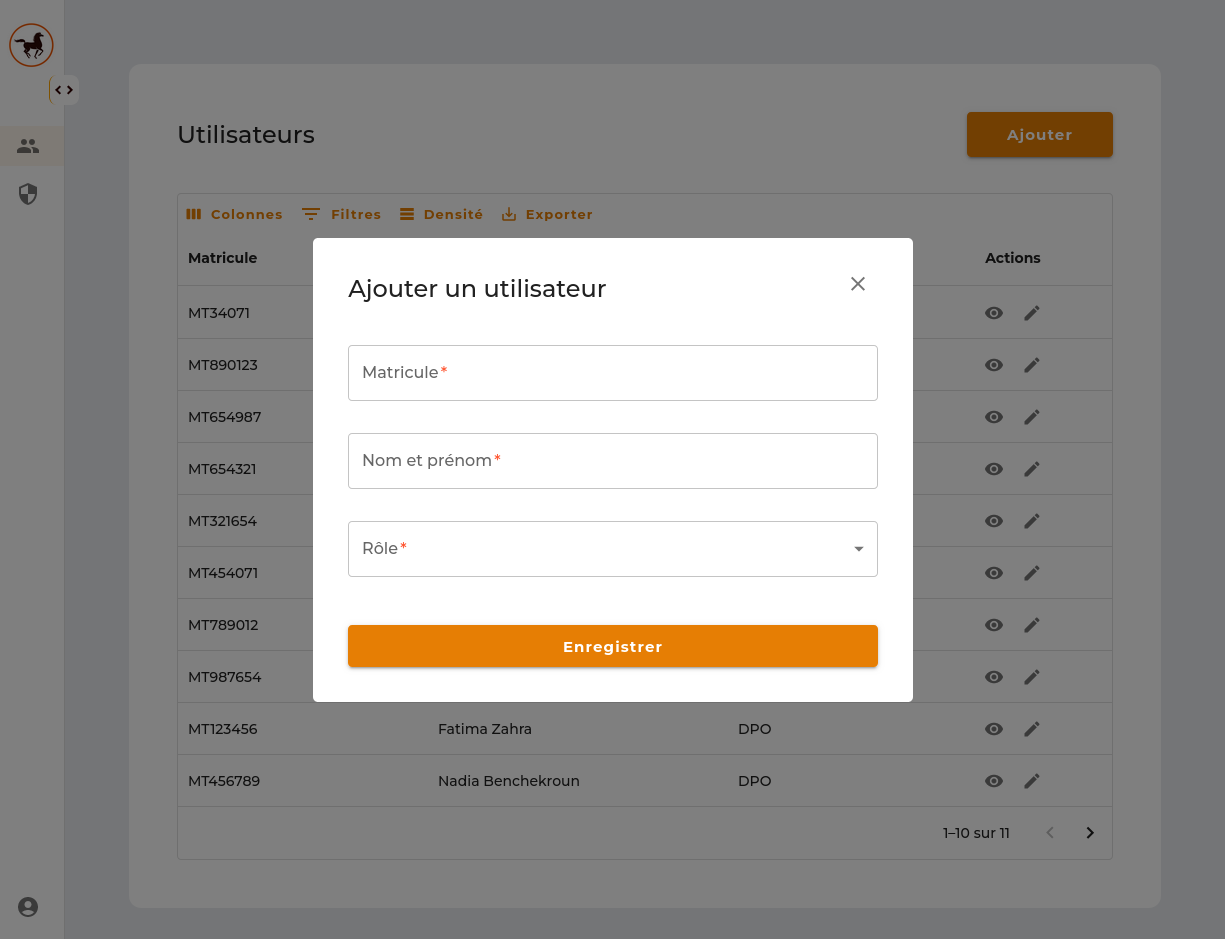
\includegraphics[width=.9\textwidth]{images/guis/utilisateurs/form/form-empty.png}
    \caption{Interface de gestion des utilisateurs}
\end{figure}

\begin{figure}[H]
    \centering
    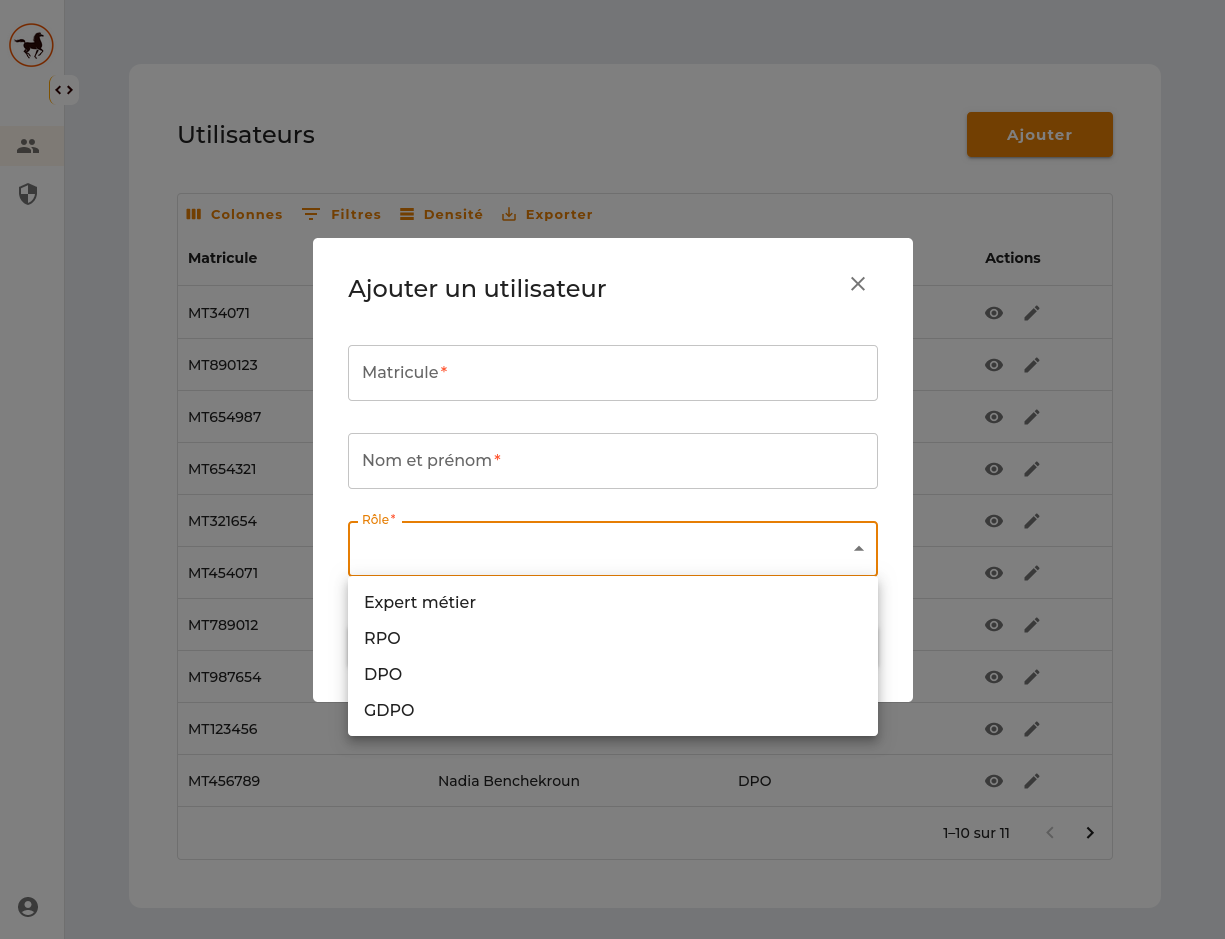
\includegraphics[width=.9\textwidth]{images/guis/utilisateurs/form/form-role-options.png}
    \caption{Interface de gestion des utilisateurs}
\end{figure}

\noindent La figure suivante démontre un exemple d'ajout d'un RPO dont le nom et prénom est "Farah Tariq" et dont le matricule est MT6543521: \\

\begin{figure}[H]
    \centering
    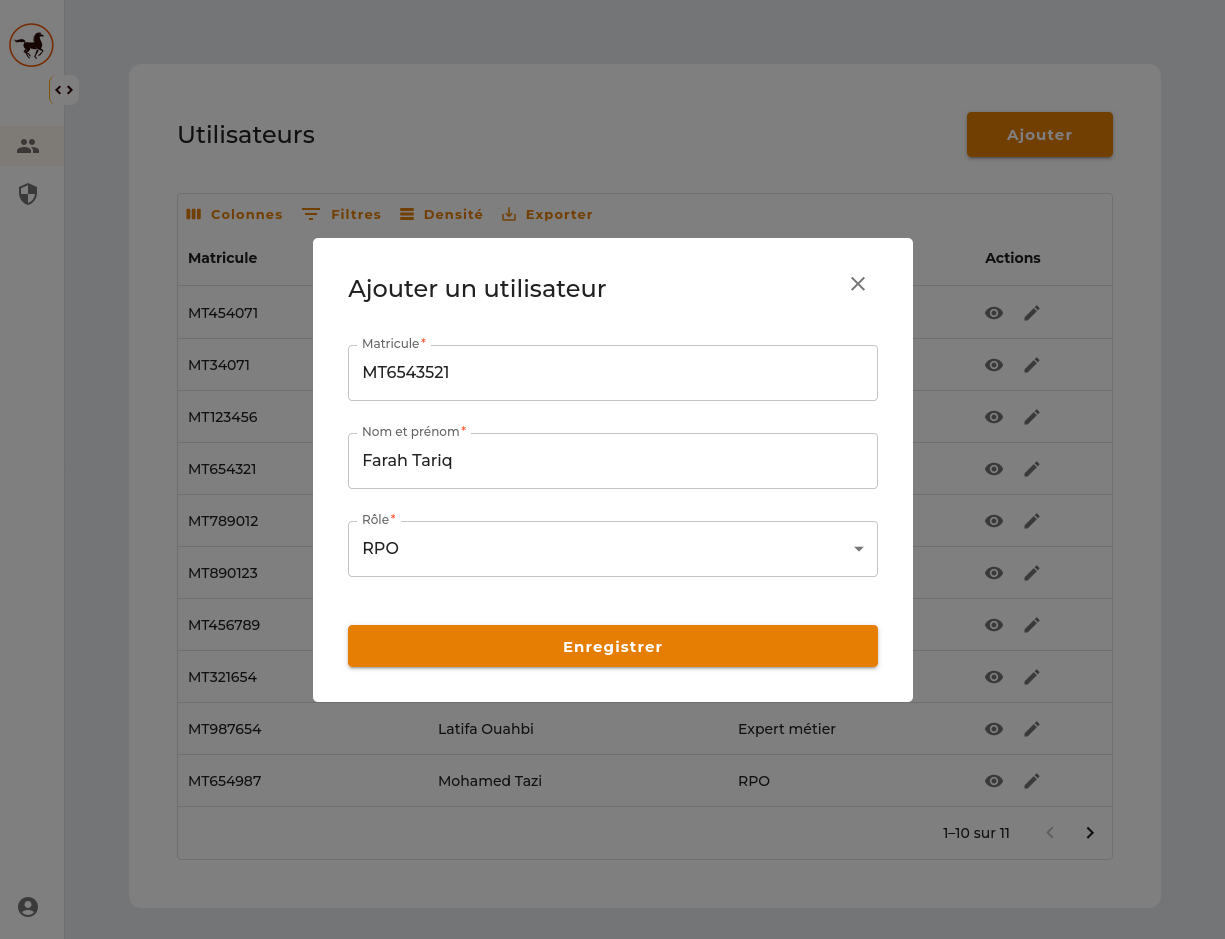
\includegraphics[width=\textwidth]{images/guis/utilisateurs/form/form-filled.png}
    \caption{Interface de gestion des utilisateurs}
\end{figure}

\noindent Suite à l'enregistrement de cet utilisateur, un alerte est affiché qui en confirme la création: \\

\begin{figure}[H]
    \centering
    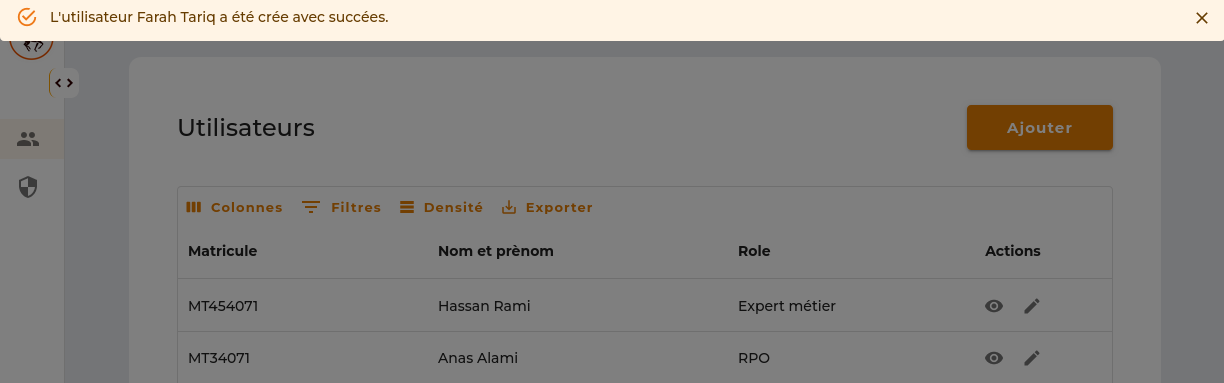
\includegraphics[width=\textwidth]{images/guis/utilisateurs/created.png}
    \caption{Interface de gestion des utilisateurs}
\end{figure}

\clearpage

\noindent Le tableau des utilisateurs s'adapte pour refleter l'enregistrement du nouveau RPO: \\

\begin{figure}[H]
    \centering
    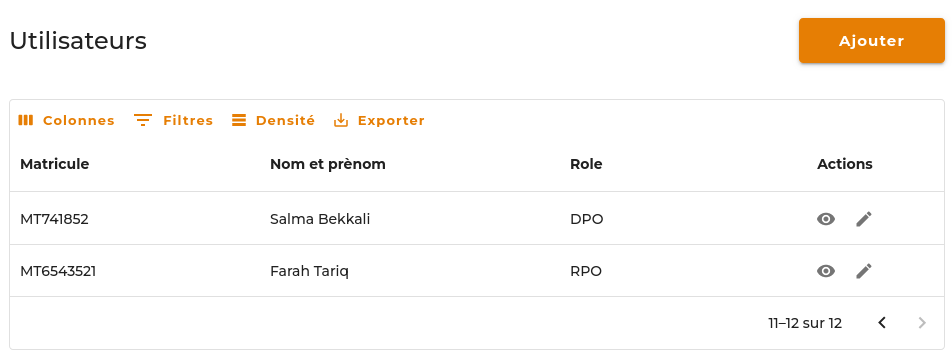
\includegraphics[width=\textwidth]{images/guis/utilisateurs/table-post-creation.png}
    \caption{Interface de gestion des utilisateurs}
\end{figure}


\subsection{Gestion des rôles}

L'interface dédiée à la gestion des roles suit une structure similaire à celles des interfaces destinées à la gestion des autres objets métier. Elle comporte un tableau listant l'ensemble des acteurs du registre de traitement et exposant la possibilité d'apporter des modifications à ces derniers en matière des permissions dont ils disposent. \\

\begin{figure}[H]
    \centering
    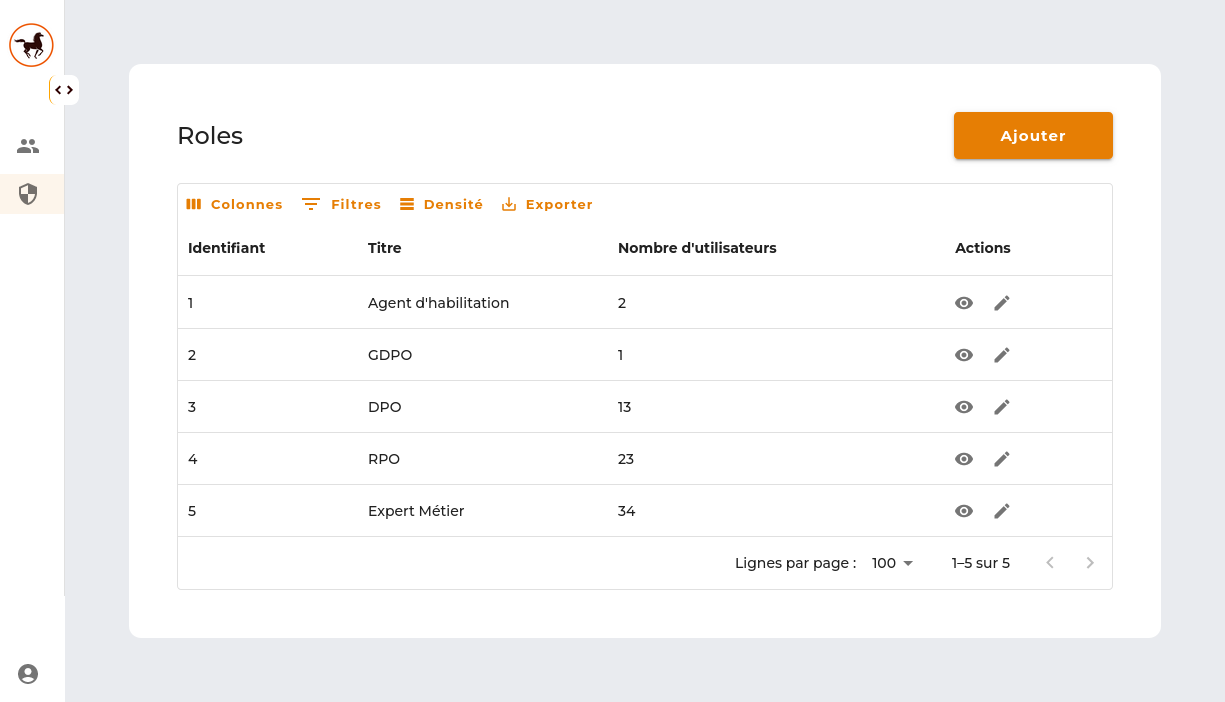
\includegraphics[width=\textwidth]{images/guis/roles.png}
    \caption{Interface de gestion des rôles}
\end{figure}

\noindent Les rôles étant fixes, l'interface n'expose pas la possibilité d'ajouter, ni de supprimer les rôles existants.

\clearpage

\subsection{Tableau de bord}

Le tableau de bord de l'application se compose de plusieurs sections utilisant des graphiques pour présenter diverses données de manière visuelle et intuitive. Ces graphiques permettent de visualiser les fiches par représentant, l'état des fiches, la répartition annuelle des fiches et le nombre de fiches par catégorie de données. \\

\begin{figure}[H]
    \centering
    \includegraphics[width=\textwidth]{images/guis/dashboard.png}
    \caption{Tableau de bord}
\end{figure}


\noindent Le tableau de bord comprend une première section avec un graphique à barres illustrant le nombre de fiches par représentant. Ce graphique montre des données pour 15 catégories de départements, telles que la "Banque commerciale", "Sécurité des personnes et des biens", et "Finances performance", avec des barres verticales colorées en orange et les étiquettes des catégories inclinées pour une meilleure lisibilité.

\begin{figure}[H]
    \centering
    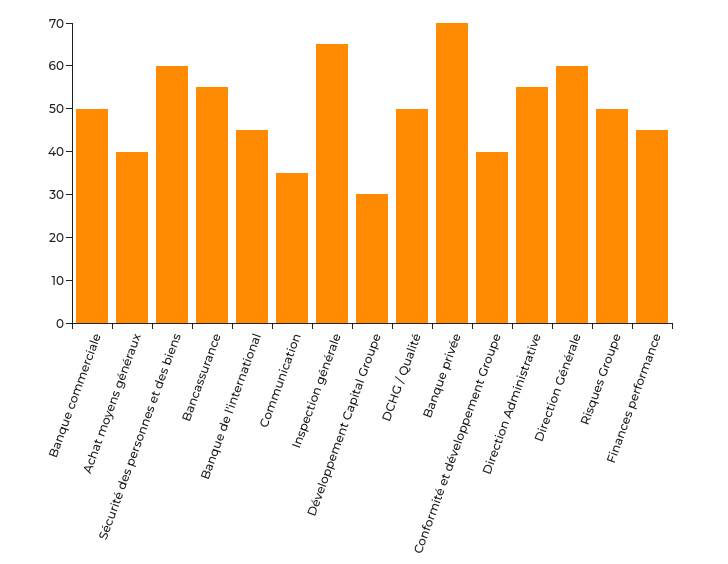
\includegraphics[width=.75\textwidth]{images/guis/dashboard1.png}
    \caption{Tableau de bord}
\end{figure}

\noindent Une autre section du tableau de bord contient un graphique en camembert représentant la partition des fiches par état. Ce graphique montre la répartition des fiches en trois segments: validées (85\%), en cours de validation (3\%) et rejetées (13\%), colorés respectivement en orange, bleu et rouge.

\begin{figure}[H]
    \centering
    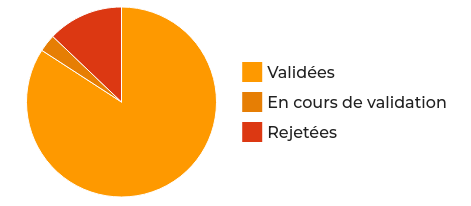
\includegraphics[width=.5\textwidth]{images/guis/dashboard2.png}
    \caption{Tableau de bord}
\end{figure}

\noindent Le tableau de bord inclut également un graphique en lignes qui affiche l'évolution annuelle du nombre de fiches créées, validées et rejetées de 2018 à 2023. Les axes X et Y représentent les années et le nombre de fiches, et les courbes colorées différencient chaque série de données : fiches créées (bleu), validées (rouge) et rejetées (violet).

\begin{figure}[H]
    \centering
    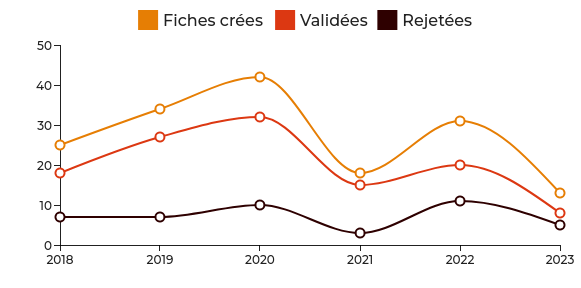
\includegraphics[width=.7\textwidth]{images/guis/dashboard3.png}
    \caption{Tableau de bord}
\end{figure}

\noindent Enfin, une section présente un autre graphique à barres montrant le nombre de fiches par catégorie de données. Ce graphique couvre 25 catégories telles que "Identification simple", "Coordonnées", et "Situation financière et patrimoniale", avec des barres rouges foncées et des étiquettes inclinées pour une meilleure visibilité.


\begin{figure}[H]
    \centering
    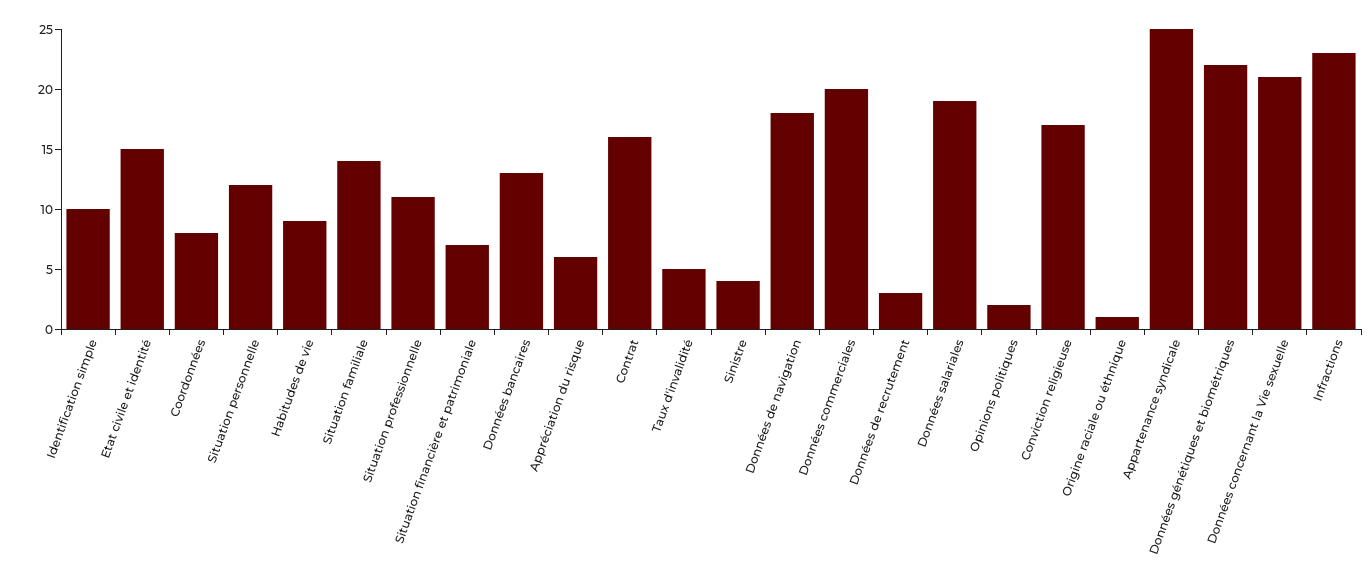
\includegraphics[width=\textwidth]{images/guis/dashboard4.png}
    \caption{Tableau de bord}
\end{figure}

\noindent Le tableau de bord de l'application utilise une variété de graphiques pour visualiser des données complexes de manière claire et attrayante. Les graphiques à barres, en camembert et en lignes offrent des aperçus détaillés et des tendances, facilitant ainsi la compréhension et la prise de décision pour les utilisateurs.
